%
% chapter.tex -- Eigenschaften Linearer Abbidungen
%
% (c) 2018 Prof Dr Andreas Müller
%
\chapter{Eigenschaften linearer Abbildungen\label{chapter:eigenschaften}}
\lhead{Lineare Abbildungen}
\rhead{}
Die bisherige Entwicklung der Vektorgeometrie hat sich vor allem auf
die geometrischen Objekte selbst konzentriert. 
Die linearen Abbildungen sind dabei nur nebenher studiert worden.
In diesem Kapitel untersuchen wir etwas genauer, wie sich lineare Abbildungen
auf das Skalarprodukt und die Orientierung auswirken und lernen die
wichtigsten Matrizengruppen kennen.

Lineare Abbildungen treten nicht nur im geometrischen Zusammenhang auf.
In vielen Gebieten der Mathematik spielen lineare Abbildungen eine
bedeutende Rolle.
Im ersten Abschnitt zeigen wir daher weitere Beispiele von linearen
Abbildungen in der Analysis.
Schliesslich zeigen wir in Abschnitt~\ref{section:kamera}, wie sich
Bilder von Kameras mit Hilfe der linearen Algebra verstehen und auswerten
lassen.

%
% linabb.tex
%
% (c) 2018 Prof Dr Andreas Müller, Hochschule Rapperswil
%
\section{Lineare Abbildungen}
\rhead{Lineare Abbildungen}
\subsection{Definition}
Eine $m\times n$-Matrix $A$ berechnet aus einem gegeben Vektor
$v\in\mathbb R^n$ mit Hilfe des
Matrizenproduktes einen neuen Vektor $Av\in\mathbb R^m$.
$A$ definiert also auch eine Abbildung
\[
A\colon\mathbb R^n\to\mathbb R^m:v\mapsto Av
\]
mit den Eigenschaften
\[
\left.
\begin{aligned}
A(u+v)&=Au+Av\\
A(\lambda u)&=\lambda Au
\end{aligned}\right\}\quad
\Rightarrow\quad
A(\lambda u+\mu v)=\lambda Au+\mu Av.
\]
Eine solche Abbildung heisst linear.
\index{lineare Abbildung}

\subsection{Matrix einer linearen Abbildung}
Umgekehrt definiert jede lineare Abbildung $V\to V$ mit Hilfe einer
Basis auch eine Matrix.
Sei $\varphi\colon V\to V$ eine Abbildung
mit $\varphi(\lambda u+\mu v)=\lambda \varphi(u)+\mu\varphi(v)$,
und $B=\{b_1,\dots,b_n\}$ eine Basis.
Dann genügt die Kenntnis
von $\varphi(b_i)$ für alle $i$, um die lineare Abbildung für
jeden beliebigen Vektor berechnen zu können.

Man kann nämlich jeden Vektor mit Hilfe seiner Koordinanten aus
den Basisvektoren linear kombinieren, also gilt auch
\[
\varphi(v)
=
\varphi(\xi_1b_1+\dots+\xi_nb_n)
=
\xi_1\varphi(b_1)+\dots+\xi_n\varphi(b_n).
\]
Ausserdem kann man die Koordinaten von $\varphi(b_i)$ in der Basis
$B$ ermitteln, und diese Koordinatenvektoren in eine Matrix $A$
schreiben.
Dann ist $A\xi$ der Koordinatenvektor von $\varphi(v)$.
Die Matrix $A$ enthält also in den Spalten die Bilder der Basisvektoren.

\subsection{Basiswechsel}
Wie sieht die Matrix einer linearen Abbildung aus, wenn man statt
der Basis $B$ die Basis $B'$ verwendet? Sei $T$ die Transformationsmatrix,
die Koordinaten bezüglich $B$ in Koordinaten bezüglich $B'$ umrechnet.
Die lineare Abbildung hat bezüglich der Basis $B$ die Matrix $A$, wir
suchen aber die Matrix $A'$, die die lineare Abbildung bezüglich der
Basis $B'$ beschreibt:
\[
\xymatrix{
\mathbb R^n\ar[r]^{A} \ar[d]_{T}
	&\mathbb R^n \ar[d]^{T}
\\
\mathbb R^n\ar[r]^{A'}
	&\mathbb R^n
}
\]
Aus dem Diagramm können wir ablesen, dass $A'$ gleichbedeutend
ist damit, die Koordinaten zuerst mit $T^{-1}$ von der Basis $B'$
auf die Basis $B$ umzurechnen, dort die Matrix $A$ anzuwenden, und
dann erneut mit $T$ in die Basis $B'$ zurückzukehren:
\begin{equation}
A'=TAT^{-1}.
\label{abbildung-basiswechsel}
\end{equation}


%
% bildkern.tex
%
% (c) 2018 Prof Dr Andreas Müller, Hochschule Rapperswil
%
\section{Bild und Kern\label{section:bildundkern}}
\rhead{Bild und Kern}
In Kapitel~\ref{chapter-lingl} wurde die Lösungsmenge eines linearen
Gleichungssystems mit der Matrix $A$ untersucht.
In Kapitel~\ref{chapter:affin} 
haben wir einer Matrix $A$ auch eine geometrische Bedeutung
als Abbildungsmatrix gegeben.
Die Frage der Lösbarkeit von Gleichungssystemen und der Begriff des
Ranges sollten daher auch eine geometrische Aussage übersetzt
werden können, was wir in diesem Abschnitt tun wollen.

\subsection{Bildraum}
Die Matrix $A$ einer linearen Abbildung $\varphi$ enthält in den Spalten
die Bilder der Standardbasisvektoren.
Vektoren, die als Bilder der Abbildung $\varphi$ auftreten können,
müssen Linearekombinationen der Spaltenvektoren von $A$ sein.
\begin{definition}
Die {\em Bildmenge} $\operatorname{im}\varphi$ einer linearen Abbildung
$\varphi$ ist der Vektorraum
\[
\operatorname{im}\varphi
=
\{\varphi(v)\;|\;v\in\mathbb R^n\}.
\]
\end{definition}

Die Bildmenge $\operatorname{im}\varphi$ der Abbildung $\varphi$ ist
daher nichts anderes als die Menge aller möglichen Linearkombinationen
von Spaltenvektoren.
Diese haben wir Seite \pageref{skript:affin:koordinaten:aufgespannt}
als den erzeugten Raum der Spaltenvektoren kennengelernt.
Wir fassen zusammen:
\begin{satz}
Die Bildmenge einer linearen Abbildung $\varphi$ ist der von den
Spaltenvektoren der zugehörigen Abbildungsmatrix $A$ aufgespannte Raum:
\[
\operatorname{im}\varphi
=
\langle\vec{a}_1,\dots,\vec{a}_n\rangle
=
\langle\mathcal{A}\rangle,
\]
wobei $\mathcal{A}$ für die Menge der Spaltenvektoren von $A$ geschrieben
haben.
\end{satz}

\subsection{Lösbarkeit von Gleichungssystemen}
Ein Gleichungssystem mit Koeffizientenmatrix $A$ und rechter Seite $b$
ist lösbar genau dann, wenn es einen Spaltenvektor $x$ gibt, derart
dass $Ax=b$.
Das Gleichungssystem ist also genau dann lösbar, wenn die rechte Seite
im Bildraum von $A$ liegt.

\begin{beispiel}
Ist der Vektor
\[
b=\begin{pmatrix}4\\2\\4\end{pmatrix}
\qquad\text{im Bildraum der Abbildung mit Matrix}\qquad
A=
\begin{pmatrix}
  -43& -26&  56\\
  -22& -12&  28\\
  -44& -26&  57
\end{pmatrix}\text{?}
\]
Die Frage ist gleichbedeutend damit, ob das Gleichungsystem mit
Koeffizientenmatrix $A$ und rechter Seite $b$ lösbar ist.
Das Gauss-Tableau
\[
\begin{tabular}{|>{$}c<{$}>{$}c<{$}>{$}c<{$}|>{$}c<{$}|}
\hline
  -43& -26&  56&4\\
  -22& -12&  28&2\\
  -44& -26&  57&4\\
\hline
\end{tabular}
\quad\rightarrow\quad
\begin{tabular}{|>{$}c<{$}>{$}c<{$}>{$}c<{$}|>{$}c<{$}|}
\hline
   1&  0& -1&  0\\
   0&  1& -\frac12&   0\\
\hdashline
   0&  0&  0&  1\\
\hline
\end{tabular}
\]
zeigt, dass dies wegen der $1$ in der rechten unteren Ecke nicht möglich
ist.
\end{beispiel}

\subsection{Dimension des Bildraumes}
Der Bildraum ist der von den Spaltenvektoren der Abbildungsmatrix
aufgespannte Raum.
Es kann durchaus sein, dass nicht alle Spaltenvektoren linear unabhängig
sind, die Dimension des Bildraumes kann also auch kleiner sein also die
Anzahl der Spaltenvektoren.

\begin{aufgabe}
Wie gross ist die Dimension des Bildraumes einer linearen Abbildung
$\varphi$ mit Abbildungsmatrix $A$?
\end{aufgabe}
Die Dimension eines Vektorraumes ist die maximale Anzahl linear
unabhängiger Vektoren einer Basis.
Da die Spaltenvektoren von $A$ alles erzeugen, müssen wir nur noch
ein paar Vektoren weglassen, welche nicht linear unabhängig sind von
den anderen.
In Kapitel~\ref{chapter-lingl} haben wir gelernt, dass der Rang der
Matrix $A$ genau die Anzahl der linear unabhängigen Spalten ist.
er ist daher auch die Dimension des Bildraumes.

\begin{satz}
Ist $A$ die Abbildungsmatrix einer linearen Abbildung $\varphi$, dann
gilt
\[
\dim\operatorname{im}\varphi = \operatorname{Rang}A.
\]
\end{satz}

\subsection{Nullmenge}
\begin{definition}
Sei $\varphi$ eine lineare Abbildung.
Die Menge
\[
\operatorname{ker}\varphi = \{\vec{v}\;|\; \varphi(\vec{v}) = 0\}
\]
heisst {\em Nullmenge}, {\em Nullraum} oder {\em Kern} der Abbildung
$\varphi$.
\end{definition}

Der Kern von $\varphi$ ist ein Vektorraum, denn wenn zwei Vektoren
$\vec{u},\vec{v}\in\ker\varphi$ im Kern sind, dann gilt dies
auch für die Summe und für die Vielfachen:
\[
\begin{aligned}
\varphi(\vec{u}+\vec{v})
&=
\varphi(\vec{u})+\varphi(\vec{v})
=
0+0=0
&&\Rightarrow&
\vec{u}+\vec{v}&\in\ker\varphi
\\
\varphi(\lambda\vec{u})
&=
\lambda\varphi(\vec{u}) = \lambda\cdot 0=0
&&\Rightarrow&
\lambda\vec{u}&\in\ker\varphi
\end{aligned}
\]
Damit stellt sich automatisch die folgende Aufgabe.

\begin{aufgabe}
Sei $\varphi$ eine lineare Abbildung mit Abbildungsmatrix $A$.
Man finde eine Basis von $\ker\varphi$.
\end{aufgabe}

Der Kern besteht aus denjenigen Vektoren $\vec{x}$, die $A\vec{x}=0$
erfüllen.
Der Kern von $\varphi$ ist daher nichts anderes als die Lösungsmenge
des Gleichungssystems $Ax=0$, welche man mit dem Gauss-Algorithmus
bestimmen kann, wie in Abschnitt~\ref{section:loesungsmenge} gezeigt
wurde.
Dort wurde auch gezeigt, dass die Anzahl der frei wählbaren Variablen
auch die Anzahl der Basisvektoren der Lösungsmenge ist.
Wenn $A$ eine $m\times n$-Matrix ist mit $\operatorname{Rang}A=r$,
dann ist die Anzahl der frei wählbaren Variablen $n-r$, es gilt
also
\[
\dim\ker \varphi = n -\operatorname{Rang}A.
\]

\begin{beispiel}
Man finde eine Basis des Kernes der linearen Abbildung mit Matrix
\[
A=\begin{pmatrix}
    9& -31& -26&   0\\
    2& -10& -12& -28\\
    8& -29& -26& -13
\end{pmatrix}
\]
\smallskip

{\parindent0pt Das} zugehörige Tableau ist
\begin{equation}
\begin{tabular}{|>{$}c<{$}>{$}c<{$}>{$}c<{$}>{$}c<{$}|>{$}c<{$}|}
\hline
    9& -31& -26&   0&0\\
    2& -10& -12& -28&0\\
    8& -29& -26& -13&0\\
\hline
\end{tabular}
\quad\rightarrow\quad
\begin{tabular}{|>{$}c<{$}>{$}c<{$}>{$}c<{$}>{$}c<{$}|>{$}c<{$}|}
\hline
    1&   0&   4&  31&0\\
    0&   1&   2&   9&0\\
\hdashline
    0&   0&   0&   0&0\\
\hline
\end{tabular}
\label{skript:affin:kern:tableau}
\end{equation}
Die letzten zwei Variablen sind frei wählbar, wir nennen sie $x_3$ und $x_4$,
dann wird die Lösungsmenge
\[
\ker\varphi
=
\mathbb L
=
\left\{
\left.
x_3
\begin{pmatrix}
-4\\-2\\1\\0
\end{pmatrix}
+
x_4
\begin{pmatrix}
-31\\-9\\0\\1
\end{pmatrix}
\;
\right|
\;
x_3,x_4\in\mathbb R
\right\}.
\]
Der Kern von $\varphi$ ist also ein zweidimensionaler Raum mit der Basis
\[
\mathcal{B} = \left\{
\begin{pmatrix}
-4\\-2\\1\\0
\end{pmatrix},
\begin{pmatrix}
-31\\-9\\0\\1
\end{pmatrix}
\right\}.
\]
Das Tableau \eqref{skript:affin:kern:tableau} zeigt auch, dass
$\operatorname{Rang}A=2$,
passend zur Dimension $\dim\ker\varphi = n - \operatorname{Rang}A = 4-2=2$ von
$\ker\varphi$.
\end{beispiel}



%
% gruppen.tex
%
% (c) 2018 Prof Dr Andreas Müller, Hochschule Rapperswil
%
\section{Gruppen\label{section:gruppen}}
\rhead{Gruppen}
Gleichungen lösen beruht darauf, dass sich Rechenoperationen rückgängig
machen lassen.
Zum Beispiel kann man in den reellen Zahlen Additionen und Multiplikationen
rückgängig machen, wenigstens wenn der Faktor nicht $0$ ist.
Im Vektorraum $\mathbb R^n$ können Additionen und
Multiplikationen mit reellen Zahlen rückgängig gemacht werden.
Das Vektorprodukt in $\mathbb R^3$ kann jedoch nicht rückgängig gemacht
werden, da verschiedene Faktoren auf das gleichen Produkt führen können.
Es gilt zum Beispiel
\[
\vec{a} \times (\vec{b} + t\vec{a})
=
\vec{a} \times \vec{b} + t(\underbrace{\vec{a}\times\vec{a}}_{\displaystyle=0})
=
\vec{a} \times \vec{b},
\]
für beliebige Werte von $t$ entsteht also immer das gleiche Produkt.
Daher ist es nicht möglich, aus dem Produkt mit $\vec{a}$ den
zweiten Faktor zurückzugewinnen.
Eine Gruppe ist eine Menge von mathematischen Objekten mit einer
Operation, die sich immer rückgängig machen lässt.

In diesem Abschnitt beschreiben wir die Eigenschaften der linearen
Abbildungen, die wir in früheren Kapiteln kennengelernt haben und
zeigen, dass sie alle Gruppen bilden.

%
% Was ist eine Gruppe
%
\subsection{Was ist eine Gruppe?}
\begin{definition}
Eine Gruppe $G$ ist eine Menge mit einer Verknüpfung, die meistens
multiplikativ geschrieben wird, und die folgende Eigenschaften hat:
\begin{enumerate}
\item Die Verknüpfung ist assoziativ: $a(bc)=(ab)c$ für alle $a,b,c\in G$.
\item Es gibt ein Element $e\in G$, genannt das neutrale Element,
mit der Eigenschaft $ae=ea=a$ für alle
Elemente $a\in G$.
\item Zu jedem Element $a$ gibt es ein Element $a^{-1}\in G$, genannt
das inverse Element von $a$, mit der
Eigenschaft, dass $a^{-1}a=e$.
\end{enumerate}
\end{definition}

Schreibt man die Verknüpfung additiv, dann können die Axiome für
eine Gruppe wie folgt geschrieben werden.
\begin{enumerate}
\item Die Verknüpfung ist assoziativ:
$a+(b+c)=(a+b)+c$ für $a,b,c\in G$.
\item Es gibt ein Element $0\in G$, genannt das neutrale Element oder
das Nullelement, mit der Eigenschaft $0+a=a+0=a$ für alle Elemente $a\in G$.
\item Zu jedem Element $a\in G$ gibt es ein Element $-a\in G$, genant
das negative Element von $a$, mit der Eigenschaft, dass $-a + a=0$.
\end{enumerate}

\begin{beispiel}
Die nicht verschwindenden reellen Zahlen
$\mathbb R^*=\{x\in\mathbb R\;|\; x\ne 0\}$
ist eine Gruppe mit der Multiplikation als Verknüpfung.

\smallskip

{\parindent0pt Das neutrale} Element ist die Zahl $1$, das inverse Element
von $a\in\mathbb R^*$ ist $1/a$.
\end{beispiel}

\begin{beispiel}
Die reellen Zahlen $\mathbb R$ mit der Addition als Verknüpfung ist eine
Gruppe.
\end{beispiel}

\begin{beispiel}
Ein Vektorraum $V$ ist eine Gruppe bezüglich der Verknüpfung der Addition
von Vektoren.
\end{beispiel}

%
% die allgemeine lineare Gruppe
%
\subsection{Die allgemeine lineare Gruppe $\operatorname{GL}_n(\mathbb R)$}
Die Menge der Matrizen $M_{mn}(\mathbb R)$ bildet keine Gruppe.
Zunächst ist die Multiplikation von Matrizen in $M_{mn}(\mathbb R)$
nicht definiert, ausser wenn $m=n$ gilt.
Für $m=n$ ist ein neutrales Element leicht zu finden.
Die Einheitsmatrix $E$ hat die Eigenschaft $AE=EA=A$.
Um eine Gruppe zu erhalten, muss man sich zusätzlich auf die 
Matrizen beschränken, welche invertierbar sind.

\begin{definition}
Die allgemeine lineare Gruppe ist die Menge
\[
\operatorname{GL}_n(\mathbb R)
=
\{ A\in M_n(\mathbb R)\;|\; \text{$A$ ist invertierbar}\}.
\]
\end{definition}

Für $n=1$ ist $\operatorname{GL}_1(\mathbb R) = \mathbb R^*
= \mathbb R\setminus \{0\}$, die invertierbaren reellen Zahlen.
Um zu entscheiden, ob eine Matrix invertierbar ist, kann die Determinante
verwendet werden.
Die Determinante ist eine Abbildung
\[
\det
\colon
M_n(\mathbb R) \to \mathbb R
:
A \mapsto \det(A).
\]
Die allgemeine lineare Gruppe besteht aus denjenigen Matrizen,
die eine von $0$ verschiedene Determinante haben.
Das sind genau die Matrizen, die von der Determinante
auf einen Wert in $\mathbb R^*$ abgebildet werden.
Die Determinante ist daher eine surjektive Abbildung
\[
\det
\colon
\operatorname{GL}_n(\mathbb R)
\to
\mathbb R^*.
\]

Die Produktregel für die Determinante besagt, dass 
\begin{align*}
\det(AB)&=\det(A)\det(B),
\\
\det(A^{-1})&=\det(A)^{-1}.
\end{align*}
Die Determinante ist daher verträglich mit den Gruppenoperationen
von $\operatorname{GL}_n(\mathbb R)$ und $\mathbb R^*$.

%
% orthogonale Gruppe
%
\subsection{Die orthogonale Gruppe $\operatorname{O}(n)$
\label{subsection:orthogonale gruppe}}
Orthogonale Matrizen sind immer invertierbar, denn $A^t$ ist die 
inverse Matrix zu einer orthogonalen Matrix $A$.
Die orthogonalen Matrizen bilden daher eine Teilmenge der invertierbaren
Matrizen, die sogenante orthogonale Gruppe.

\begin{definition}
Die Menge aller orthogonalen Matrizen
\[
\operatorname{O}(n) = \{ A\in M_n(\mathbb R)\;|\; AA^t = E \}
\subset \operatorname{GL}_n(\mathbb R)
\]
heisst die orthogonale Gruppe.
\end{definition}
Die orthogonale Gruppe enthält einerseits alle Drehmatrizen, aber auch
alle Spiegelungen, da diese ebenfalls das Skalarprodukt erhalten.
Des Weiteren sind Produkte von Drehmatrizen und Spiegelungsmatrizen
ebenfalls in $\operatorname{O}(n)$.

Aus der Produktformel für die Determinante folgt
\[
A^tA=E
\quad\Rightarrow\quad
1
=
\det(E)
=
\det(A^tA)
=
\det(A^t)\det(A)
=
\det(A)^2
\quad\Rightarrow\quad
\det(A)=\pm 1.
\]
Orthogonale Matrizen haben also immer Determinante $\pm 1$.
Sie erhalten
also auf jeden Fall das Volumen, aber nicht unbedingt das orientierte
Volumen.
Spiegelungen kehren offensichtlich das Volumen um, sie haben Determinante
$-1$.

%
% spezielle lineare Gruppe
%
\subsection{Die spezielle lineare Gruppe $\operatorname{SL}_n(\mathbb R)$}
Matrizen in der allgemeinen linearen Gruppe $\operatorname{GL}_n(\mathbb R)$
können das Volumn verändern oder die Orientierung umkehren.
Die Orientierung oder das orientiert Volumen werden nur dann erhalten
sein, wenn die Determinante $1$ ist.

\begin{definition}
Die spezielle lineare Gruppe ist
\[
\operatorname{SL}_n(\mathbb R)
=
\{ A\in\operatorname{GL}_n(\mathbb R) \;|\; \det (A)=1\}.
\]
\end{definition}

Tatsächlich ist diese Menge eine Gruppe.
Dazu müssen wir überprüfen, dass das Produkt von Matrizen in
$\operatorname{SL}_n(\mathbb R)$
wieder in
$\operatorname{SL}_n(\mathbb R)$
ist.
Dies folgt aber aus der Produkteigenschaft der Determinante:
\[
\det(AB) 
=
\det(A) \det(B)
=
1\cdot 1
=
1
\]
für $A,B\in\operatorname{SL}_n(R)$.
Analog folgt auch, dass $A^{-1}\in\operatorname{SL}_n(\mathbb R)$ wenn
$A\in\operatorname{SL}_n(\mathbb R)$.

%
% Gruppe der Drehmatrizen
%
\subsection{Die Drehgruppe $\operatorname{SO}(n)$}
Drehungen des Raumes sind lineare Abbildungen, die 
das Skalarprodukt und die Orientierung erhalten.
Sie bilden die {\em spezielle orthogonale Gruppe}
\[
\operatorname{SO}(n) 
=
\operatorname{O}(n) \cap \operatorname{SL}_n(\mathbb R)
=
\{
A\in M_n(\mathbb R)\;|\; A^tA=E\wedge \det(A) = 1
\}.
\]

Die Differenz $\operatorname{O}(n) \setminus \operatorname{SO}(n)$
besteht aus Matrizen, die zwar das Skalarprodukt erhalten, aber die
Orientierung umkehren.
Ist $S_x$ die Spiegelung an der Ebene senkrecht zur $x$-Achse und ist
$A\in \operatorname{O}(n) \setminus \operatorname{SO}(n)$, dann ist
\[
\det(S_xA)= \det(S_x)\det(A) = (-1)\cdot(-1)=1
\qquad\Rightarrow\qquad
S_xA\in\operatorname{SO}(n).
\]
Dies bedeutet, dass die Multiplikation mit $S_x$ eine bijektive Abbildung
\[
\operatorname{SO}(n) \to \operatorname{O}(n)\setminus\operatorname{SO}(n)
:
A\mapsto S_xA
\]
definiert.
Die Gruppe $\operatorname{O}(n)$ besteht also aus zwei gleichartig gebauten
Teilmengen, $\operatorname{SO}(n)$  und
$\operatorname{O}(n)\setminus\operatorname{SO}(n)$.

Man kann die Gruppe $\operatorname{SO}(3)$ die Gruppe der Robotik nennen,
denn bei allen Bewegungen, die ein Roboter im Raum ausführen kann,
bleiben die Abmessungen erhalten (er soll ja nicht deformiert werden)
und die Orientierung kann nicht umkehren.
Die Bewegung eines Roboters besteht daher immer aus einer
Translationskomponente und einer Drehung in $\operatorname{SO}(3)$.
Die Herausforderung dabei ist natürlich, dass die Gruppe
$\operatorname{SO}(3)$ ziemlich kompliziert und vor allem nicht
kommutativ ist.

Für die Beschreibung einer Drohne ist es unabdingbar, in der
Gruppe $\operatorname{SO}(3)$ arbeiten zu können.
Wenn man die Bewegung eines Roboters aber weiter einschränken kann,
zum Beispiel indem man nur Bewegungen in der Ebene und Drehungen
um eine vertikale Achse zulässt, wie dies zum Beispiel bei
Eurobot gemacht wird, dann reicht es mit der Gruppe der Verschiebungen
und zweidimensionalen Drehungen um $\operatorname{SO}(2)$ zu arbeiten.
Diese letzte Gruppe ist viel einfacher, da sich Drehungen in der Ebene
durch den Drehwinkel beschreiben lassen und die Gruppe daher kommutativ ist.



%\begin{verbatim}
5.1 Determinante und Orientierung
- Orientierter Flächeninhalt
- Orientiertes Volumen
5.2 Vektorprodukt
- Definition und Eigenschaften
- Normalenvektoren
- Abstandsformeln
\end{verbatim}


\subsection{Wavelets\label{subsection-wavelets}}
Die Erfindung der Fourier-Reihen durch Jean-Baptiste Fourier erm"oglichte,
beliebige periodische Funktionen in ihre Frequenzkomponenten zu zerlegen,
diese einzeln zu studieren, zu modifizieren und daraus eine neue Funktion
zu synthetisieren. Fourier-Reihen und die Fourier-Transformation haben
sich zu Standardwerkzeugen sowohl in den Anwendungen wie auch in der
reinen Mathematik entwickelt.

In der Praxis kennt man von einer Funktion, die zum Beispiel in
Oszilloskop misst, die Funktionswerte nur zu diskreten Zeitpunkten,
Abbildung~\ref{signal:vector}.
Auch von solchen Funktionen kann man das Frequenz-Spektrum bestimmen.
Die theorie hat jedoch ein paar Nachteile:
\begin{compactenum}
\item Um die hochfrequenten Komponenten, also die ``Detailinformation''
"uber das Signal zu bekommen, muss man das gesamte Signal analysieren.
Man w"urde sich w"unschen, dass Detailinformationen aus einer Analyse
nur eines kurzen Zeitabschnitts des Signals ermittelbar sind.
\item "Andert man eine Frequenzkomponente, "andert sich das Signal
"uberall. Man w"urde sich w"unschen, dass "Anderungen m"oglichst nur
lokale Wirkung haben.
\end{compactenum}
Wavelets l"osen diese Probleme. Statt zeitlich ausgedehnter Sinus-
und Kosinus-Schwingungen werden nur kurze Wellenz"uge verwendet.
Je k"urzer sie sind, desto feiner die Details, die sie aus dem 
Signal analysieren. Leider ist es nicht ganz einfach, geeignete
Funktionen zu finden. Es muss viel mathematischer Aufwand getrieben
werden, damit die Wavelets m"oglichst glatt werden, nicht lange
dauern, und ausserdem das Signal m"oglichst so analysieren, dass
man damit auch praktisch n"utzliche Aufgaben l"osen kann.

Das Prinzip der Analyse eines Signals mit Wavelets kann jedoch
auch mit der Haar-Basis illustriert werden. Dies wird in diesem
Abschnitt unternommen.

\subsubsection{Signale}
\begin{figure}
\begin{center}
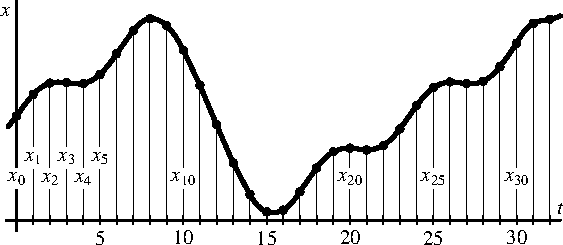
\includegraphics[width=0.9\hsize]{images/signal-1}
\end{center}
\caption{Sampling eines Signals\label{signal:vector}}
\end{figure}
Wir stellen uns ein Signal vor, welches zu einer grossen Zahl $N$
von Zeitpunkten mit gleichem Abstand abgetastet wird,
Abbildung~\ref{signal:vector}. Das Signal
wird dadurch zu einer Liste von Werten $x_1,x_1,\dots,x_N$, die
alles beinhalten, was wir "uber das Signal wissen. Ein Signal
ist also im wesentlichen ein Vektor
$$
x=\begin{pmatrix}x_1\\x_2\\\vdots\\x_N\end{pmatrix}
$$
Die Menge $\mathbb R^N$ dieser Vektoren bezeichen wir in diesem
Kapitel mit $V$. 

Die "ublichen Operationen mit Vektoren haben eine naheliegende
"Ubersetzung f"ur Signale. Die Summe zweier Vektoren entspricht
der "Uberlagerung, die Multiplikation mit einem skalaren Faktor
entspricht einer Verst"arkung des Signals. 

Ein Skalarprodukt l"asst sich wie "ublich bilden, doch ziehen
wir folgende Definition vor:
$$
x\cdot y=\sum_{i=1}^Nx_iy_i
$$
Die Vektoren $e_i$ mit $1\le i\le N$ bilden nat"urlich immer noch
eine orthonormierte Basis, diese ist jedoch f"ur die Anwendungen
nicht unbedingt gut geeignet.

Wir schreiben die Komponenten dieser Vektoren auch $x(i)$ um
eine Schreibweise zu erhalten, die "ahnlich ist der Funktionsschreibweise
f"ur eine Zeitabh"angige Funktion.

\subsubsection{Anforderungen an eine Basis}
Die Standardbasis $e_i$ passt nicht zu der Art und Weise, wie ein
Ingenieur das Signal studiert. Der Standardbasis-Vektor $e_i$
entspricht einem Peak zur Zeit $i$, zu allen anderen Zeiten
ist der Signalwert $0$.
Ein Ingenieur wird sich das Signal
typischwerweise bei verschiedenen zeitlichen Aufl"osungen
ansehen, indem er die Zeitbasis am Oszilloskop ver"andert.
Bei geringer Aufl"osung sind nur die niederfrequenten
Anteile des Signales sichtbar, bei hoher zeitlicher Aufl"osung
werden zus"atzliche Details sichtbar.
Gesucht ist daher eine Basis, die an solche Aufl"osungs"anderungen
angepasst ist.

Dem Ingenieur ist auch egal, wo innerhalb des Signals sich
ein bestimmtes Ereignis abspielt, die Basis sollte sich also
auch bei Verschiebungen entlang der Zeitachse nicht "andern.

Gesucht ist also eine alternative Basis aus Signalen, die
sich durch Zeitverschiebung und Skalierung ineinander "uberf"uhren
oder mindestens vergleichen lassen.

Die einfachsten Skalentransformationen, f"ur die wir die Basisvektoren
vorbereiten wollen, sind die zeitlichen Streckungen um den Faktor 2.
Dies wird nur m"oglich sein, wenn die Zahl $N$ gen"ugen durch $2$
teilbar ist, der Einfachheit halber setzen wir daher fest, dass
f"ur den Rest dieses Kapitels $N=2^k$.

Die Analyse eines Signals, die Zerlegung in Basisvektoren, erfordert
normalerweise die L"osung eines linearen Gleichungssystems.
Es ist unm"oglich, dies f"ur grosse Datenmengen in Echtzeit
durchzuf"uhren. Verwendet man aber eine orthonormierte Basis,
ist die Zerlegung einfach: die Koeffizienten entstehen einfach
durch Berechnung eines Skalarproduktes.

Gesucht ist jetzt also eine Basis mit folgenden Eigenschaften:
\begin{compactenum}
\item Ein Basisvektor geht in einen anderen Basisvektor "uber, wenn
man die Zeitachse um den Faktor 2 komprimiert.
\item Ein Basisvektor geht in einen anderen Basisvektor "uber, wenn
man ihn entlang der Zeitachse verschiebt, wenigstens f"ur
gewisse Offsets.
\item Die Vektoren sind orthonormiert.
\end{compactenum}
In den folgenden Abschnitten sollen diese Forderungen nach und
nach erf"ullt werden.

\subsubsection{Eine skaleninvariante Vektorfamilie}
Wir konstruieren jetzt eine Familie von Vektoren $\varphi_{i,j}$
wie folgt. $\varphi_{0,0}$ besteht aus lauter Einsen. In $\varphi_{1,j}$
ist die H"alfte der Komponenten $0$, die andere H"alfte hat den
Wert $1$. 
Diese Vektoren sind also:
\begin{align*}
\varphi_{0,0}&=\begin{pmatrix}1\\\vdots\\1\end{pmatrix}
\\
\varphi_{1,0}&=\begin{pmatrix}1\\\vdots\\1\\0\\\vdots\\0\end{pmatrix}&
\varphi_{1,1}&=\begin{pmatrix}0\\\vdots\\0\\1\\\vdots\\1\end{pmatrix}
\end{align*}
Siehe auch Abbildungen~\ref{wavelet-phi00} und \ref{wavelet-phi10-11}.
Diese Konstruktion l"asst sich fortsetzen:
\begin{align*}
\varphi_{i,j}(t)&=\begin{cases}
1&\qquad j2^{k-i}<t\le (j+1)2^{k-i}\\
0&\qquad\text{sonst}
\end{cases}
\end{align*}
Das Signal $\varphi_{i,j}$ ist also nur auf einem Abschnitt der
L"ange $2^{k-i}$ von $0$ verschieden, der Index $j$ numeriert
diese Abschnitte innerhalb der Ganzzahlen $1,\dots,2^k$.
\begin{figure}
\begin{center}
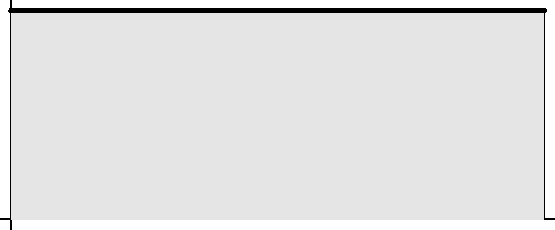
\includegraphics[width=0.45\hsize]{images/w-1}
\end{center}
\caption{Basisfunktion $\varphi_{0,0}$\label{wavelet-phi00}}
\end{figure}
\begin{figure}
\begin{center}

\includegraphics[width=0.45\hsize]{images/w-2}
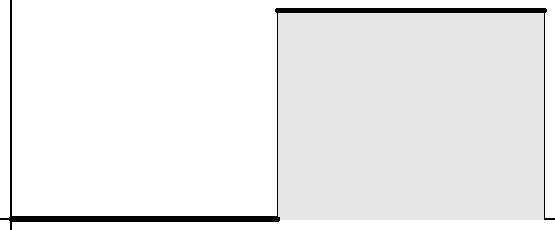
\includegraphics[width=0.45\hsize]{images/w-3}
\end{center}
\caption{Basisfunktionen $\varphi_{1,0}$ und $\varphi_{1,1}$\label{wavelet-phi10-11}}
\end{figure}

Es ist klar, dass man mit diesen Vektoren jedes beliebige Signal
darstellen kann, denn es ist ja
$\varphi_{k,j}=e_j$, die urspr"unglichen Basisvektoren geh"oren 
auch zur Familie der Funktion $\varphi_{i,j}$. Das bedeutet
aber auch, dass $\varphi_{i,j}$ keine Basis sein kann, die Familie
umfasst $2^{k+1}-1$ Vektoren, w"ahrend $V$ nur $2^k$-dimensional ist.

Die Vektoren $\varphi_{i,j}$ sind auch nicht orthogonal. Es ist
zwar $\varphi_{i,j}\cdot\varphi_{i,l}=0$ f"ur $j\ne l$. Aber es
gilt auch $\varphi_{0,0}\cdot\varphi_{i,j}=2^{k-i}$ f"ur jedes
beliebige $j$.

Lineare Abh"angigkeit kommt in der Familie $\varphi_{i,j}$ sehr
h"aufig vor. Bereits die ersten drei Vektoren sind linear
abh"angig:
$$\varphi_{0,0}=\varphi_{1,0}+\varphi_{0,1}.$$
Analoges gilt f"ur beliebige sp"ateren $\varphi$-Vektoren:
$$
\varphi_{i,j}=\varphi_{i+1,2j}+\varphi_{i+1,2j+1}
$$
Insbesondere sind also alle Vektoren $\varphi_{i,j}$ mit 
ungeradem $j$ entbehrlich. F"ur jedes $i>0$ bleiben also
nur noch $2^{i-1}$ Vektoren "ubrig, die linear unabh"angig,
sowie der Vektor $\varphi_{0,0}$. Dies sind
$$
1+\sum_{i=1}^k 2^{i-1}=1+\sum_{i=0}^{k-1}2^i=1+2^{k}-1=2^{k}=N
$$
linear unabh"angige Vektoren.

\subsubsection{Orthonormierung}
\begin{figure}
\begin{center}
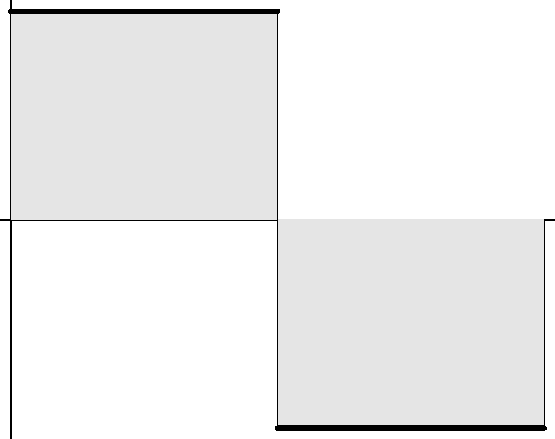
\includegraphics[width=0.45\hsize]{images/w-8}
\end{center}
\caption{Orthogonale Basisfunktion $\psi_{1,0}$\label{wavelet-psi10}}
\end{figure}

Die Vektoren $\varphi_{i,j}$ mit $j$ gerade bilden eine Basis,
mit Hilfe des Orthonormierungs-Algorithmus k"onnen Sie zu einer
orthonormierten Basis gemacht werden. Diesen Prozess verwenden
wir aber nur f"ur die Konstruktion eines ersten Vektors $\psi_{1,0}$,
und leiten daraus dann eine orthonormierte Familie ab.

Der Basisvektor $\varphi_{0,0}$ ist noch nicht
normiert, er hat L"ange $\sqrt{N}$, also ist
$$
\psi_{0,0}=\frac1{\sqrt{N}}\varphi_{0,0}
$$
der erste normierte Basisvektor.

Im zweiten Schritt muss eine Linearkombination von $\psi_{0,0}$
und $\varphi_{1,0}$ gefunden werden, welche L"ange $1$ hat und
auf $\psi_{0,0}$ senkrecht steht. Die Orthogonalit"atsbedingung
kann erf"ullt werden, indem man den Vektor
\[
v=\varphi_{1,0}-(\varphi_{1,0}\cdot\psi_{0,0})\psi_{0,0}
\]
verwendet. Da $\varphi_{1,0}\cdot\psi_{0,0}=\frac{N}2\cdot\frac1{\sqrt{N}}
=\frac1{2\sqrt{N}}$,
ergibt sich
\[
v(l)=\begin{cases}
\frac12&\qquad 0<l\le 2^{k-1}\\
-\frac12&\qquad 2^{k-1}<l\le 2^{k}
\end{cases}
\]
Dieser Vektor h"atte die L"ange $\sqrt{N\frac14}=\frac{\sqrt{N}}2$,
der orthonormalisierte Vektor ist also
\[
\psi_{1,0}=\begin{cases}
\frac1{\sqrt{N}}&\qquad l\le 2^{k-1}\\
-\frac{1}{\sqrt{N}}&\qquad 2^{k-1}<l\le 2^{k},
\end{cases}
\]
siehe auch Abbildung~\ref{wavelet-psi10}.

Mit diesem Vektor kann man jetzt alle Vektoren $\varphi_{1,j}$
darstellen:
\begin{align}
\varphi_{1,0}&=\frac12(\psi_{0,0}+\psi_{1,0})
&
\varphi_{1,1}&=\frac12(\psi_{0,0}-\psi_{1,0})
\label{psikonstruktion}
\end{align}

Jetzt konstruieren wir einen Vektor $\psi_{2,0}$. Wir schreiben $S$
f"ur die Operation des Subsampling:
\[
Sv(l)=\begin{cases}
v(2l)&\qquad 0 <l \le 2^{k-1}\\
0&\qquad 2^{k-1}<l\le N
\end{cases}
\]
Die Operation $S$ nimmt also nur jeden zweiten Wert eines Signals.
Es ist klar, dass $S\varphi_{i,0}=\varphi_{i+1,0}$ und
$S\varphi_{i,1}=\varphi_{i+1,1}$, ebenso bleiben orthogonale
Signale auch nach dem Subsampling orthogonal. Wenden wir dies
auf \ref{psikonstruktion} an, erhalten wir
\begin{align*}
S\varphi_{1,0}&=\frac12(S\varphi_{0,0}+S\psi_{1,0})
&
S\varphi_{1,1}&=\frac12(S\varphi_{0,0}-S\psi_{1,0})
\\
\varphi_{2,0}&=\frac12(\varphi_{1,0}+S\psi_{1,0})
&
\varphi_{2,1}&=\frac12(\varphi_{1,1}-S\psi_{1,0})
\end{align*}
und schliessen ausserdem, das $S\psi_{1,0}$ auf $\varphi_{1,0}$
senkrecht steht. Somit ist $S\psi_{1,0}$ ein guter Kandidat
f"ur $\psi_{2,0}$, nur die L"ange braucht noch nicht zu
stimmen. Da $S\psi_{1,0}$ jedoch f"ur genau die H"alfte der Zeitpunkte
$1$ ist, ist
$$\psi_{2,0}=\sqrt{2}S\psi_{1,0}$$
ein normierte Vektor, der senkrecht auf $\psi_{1,0}$ und $\varphi_{0,0}$
steht, Abbildung~\ref{psi2}.
\begin{figure}
\begin{center}
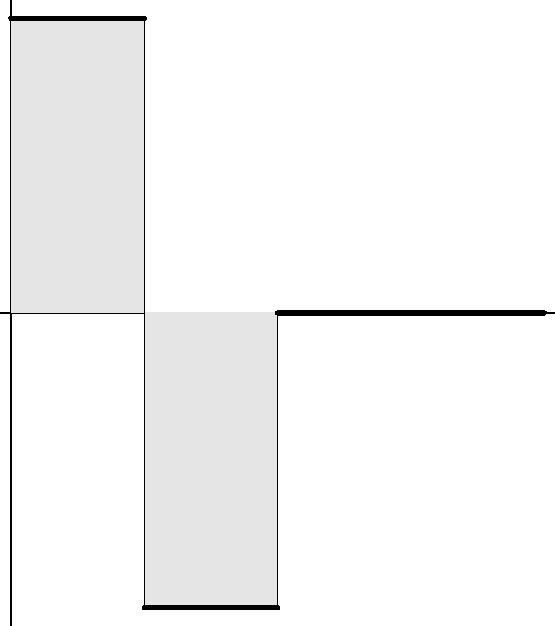
\includegraphics[width=0.45\hsize]{images/w-9}
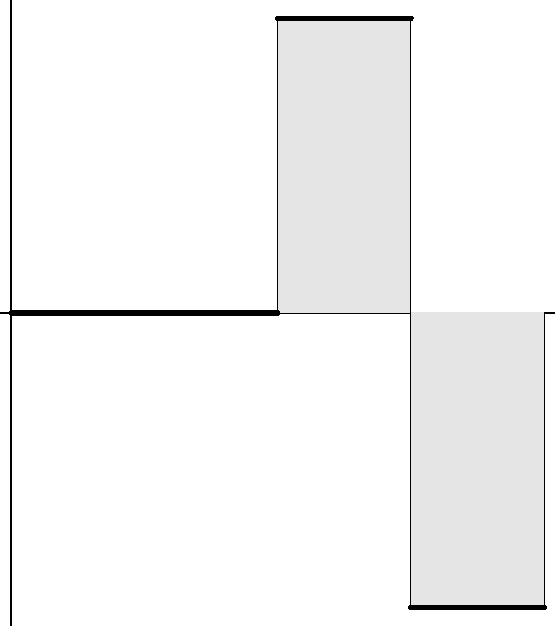
\includegraphics[width=0.45\hsize]{images/w-10}
\end{center}
\caption{Orthogonale Vektoren $\psi_{2,0}$ und $\psi_{2,1}$\label{psi2}}
\end{figure}

\begin{figure}
\begin{center}
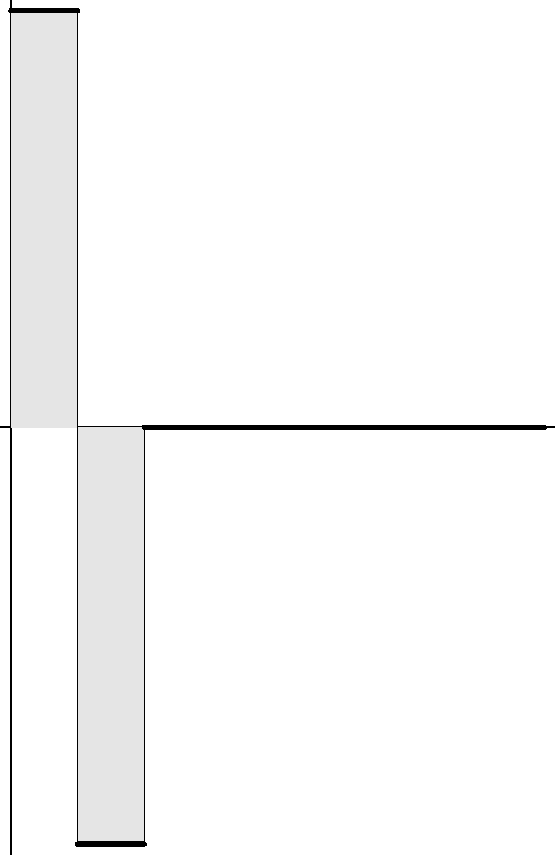
\includegraphics[width=0.22\hsize]{images/w-11}
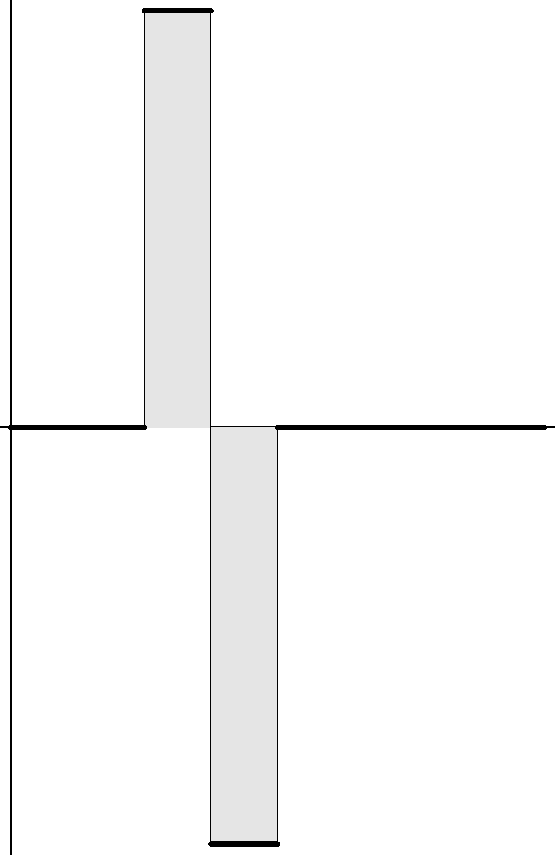
\includegraphics[width=0.22\hsize]{images/w-12}
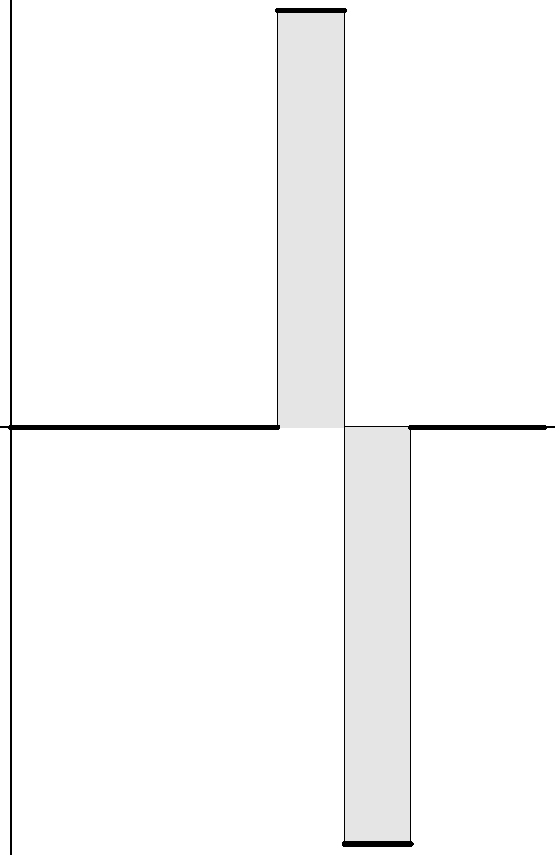
\includegraphics[width=0.22\hsize]{images/w-13}
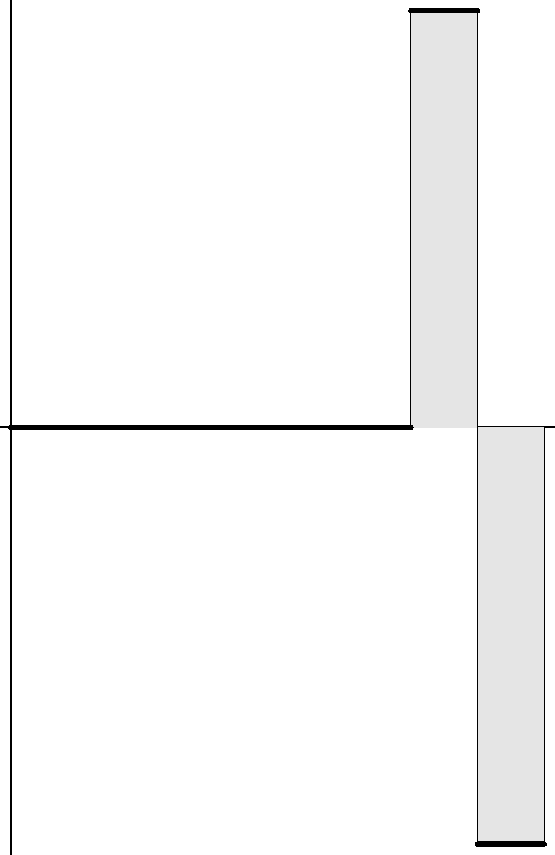
\includegraphics[width=0.22\hsize]{images/w-14}
\end{center}
\caption{Orthogonale Vektoren $\psi_{3,j}$, mit $0\le j\le 3$\label{psi3}}
\end{figure}

Ein weiterer unabh"angiger Vektor kann durch Translation gewonnen werden.
Setzen wir
$$
(T^uv)(l)=\begin{cases}
v(l-v+N)&\qquad l\le v\\
v(l-v)&\qquad l>v\\
\end{cases}
$$
f"ur die Translation um $u$ Stellen, dann ist
$$\psi_{2,1}=T^{2^{k-1}}\psi_{2,0}$$ 
ebenfalls ein Einheitsvektor und orthonormiert, das Resultat ist in Abbildung
\ref{psi2} dargestellt.

Analog kann man f"ur $\psi_{3,j}$ mit $0\le j\le 3$ vorgehen, und
erh"alt vier orthogonale Vektoren wie in Abbildung \ref{psi3}.

\subsubsection{Analyse}
Da die Vektoren $\psi_{i,j}$ mit $0\le i\le k$ und
$0\le j< 2^i$ eine orthonormierte Basis von $V$ bilden, man kann also
jeden beliebigen Vektor $v$ in dieser Basis zerlegen.
Dazu bildet man die Skalaprodukte
\begin{align*}
a_{i,j}&=\psi_{i,j}\cdot v
\end{align*}
\begin{figure}
\begin{center}
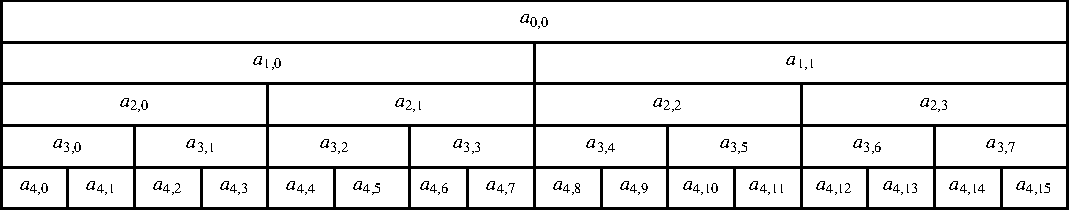
\includegraphics[width=\hsize]{images/signal-4}
\end{center}
\caption{Hierarchie der Koeffizienten $a_{i,j}$\label{coefhierarchy}}
\end{figure}
Die Berechnung der Koeffizienten ist sehr effizient m"oglich, weil die
verschiedenen Funktionen $\psi_{i,j}$ f"ur das selbe $i$ nicht gleichzeitig
von Null verschieden sind, Abbildung~\ref{coefhierarchy}.
Der Koeffizient $a_{0,0}$ ist massgebend f"ur das ganze Zeitinterval,
doch $a_{1,0}$ und $a_{1,1}$ sind je nur f"ur die H"alfte des Intervals
relevant, und brauchen auch nur Daten aus jeweils der H"alfte
des Intervals. $a_{i,j}$ wird aus Daten aus einem $2^i$-tel des
Intervals berechnet.
Die Anforderung, dass die Analyse ``lokale Detailinformation''
liefern soll, ist damit erf"ullt.

\begin{figure}
\begin{center}
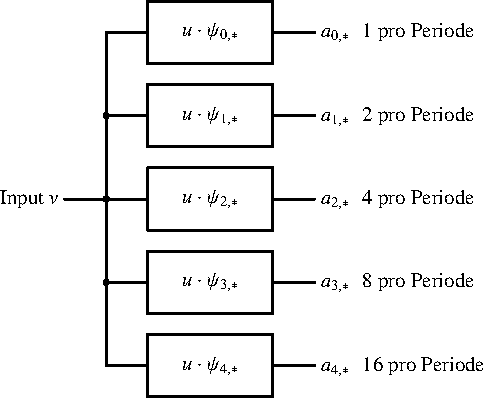
\includegraphics[width=0.65\hsize]{images/signal-2}
\end{center}
\caption{Analyse des Inputsignals $v$ mit der Basis $\{\psi_{i,j}\}$
\label{waveletanalysis}}
\end{figure}
Um den Koeffizienten von $\psi_{i,0}$ zu berechnen wird zuerst
die Summe der ersten $2^{k-i}$ Werte gebildet, dann werden die
n"achsten $2^{k-i}$ Werte subtrahiert, womit die Berechnung von $a_{i,0}$
abgeschlossen ist. Mit den nachfolgenden $2^{k-i+1}$ Werten kann dann
$a_{i,1}$ nach dem gleichen Muster berechnet werden. Mit $k$ parallelen
Recheneinheiten (Abbildung~\ref{waveletanalysis}),
die in jedem Zyklus eine Multiplikation und eine Addition zur
Bildung des Skalarproduktes durchf"uhren k"onnen\footnote{Solche 
Einheiten stehen in FPGAs als Hardwarebl"ocke zur Verf"ugung. Ebenso
implementieren Signalprozessoren genau diese Art von Operation
mit einer einzigen Instruktion.
Die Anzahl pro Sekunde ausf"uhrbarer solcher
Multiply-Accumulate-Operationen (MACs)
ist ein Leistungsmerkmal von FPGAs oder Signalprozessoren.
Man darf also davon ausgehen,
dass diese Art von Berechnung besonders effizient in angepasster
Hardware ausf"uhrbar ist, ganz im Gegensatz zum L"osen eines
Gleichungssystems.}
k"onnen also die Koeffizienten $a_{i,j}$ mit h"ochstens
einem Zyklus Verz"ogerung berechnet werden.

Der Koeffizient von $\psi_{0,0}=\varphi_{0,0}$ berechnet
den Durchschnittswert des Signals, den ``DC-Anteil''.
Der Koeffizient von $\psi_{1,0}$ gibt an, wie gross der Unterschied 
zwischen dem Durchschnittswert der beiden H"alften der Werte
des Signals sind.
Die Koeffizienten $\psi_{i,j}$ geben an, wie stark sich die Mittelwerte
von $2^{k-i}$ aufeinanderfolgenden Werten unterscheiden.
F"ur kleines $i$ werden also Mittelwerte grosser Intervalle
gebildet, und damit hochfrequente Schwankungen ausgemittelt.
Die verschiedenen Koeffizienten $a_{i,j}$ sind also ein Mass
daf"ur, wie stark verschieden hohe Frequenzen im Signal
vertreten sind. Trotzdem geht die Information nicht verloren,
wann eine Signal"anderung passiert.

\subsubsection{Synthese}
\begin{figure}
\begin{center}
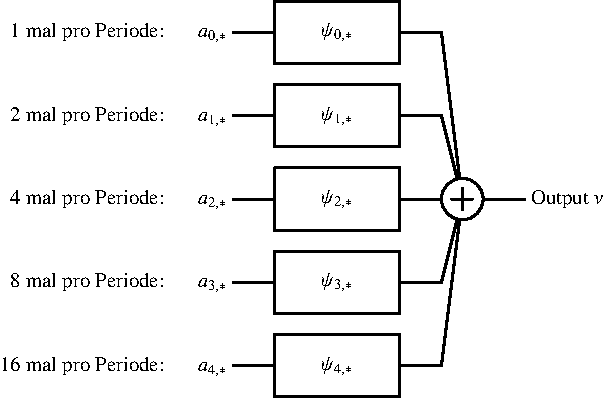
\includegraphics[width=0.8\hsize]{images/signal-3}
\end{center}
\caption{Synthese des Signals $v$ aus den Koeffizienten $a_{i,j}$
\label{waveletsynthesis}}
\end{figure}
Das urspr"ungliche Signal kann aus den Koeffizienten zur"uckgewonnen werden,
indem die Summe
$$
v=a_{0,0}\varphi_{0,0}+\sum_{i=1}^k\sum_{j=0}^{2^i-1}a_{i,j}\psi_{i,j}
$$
gebildet wird. 
Auch diese Summe kann sehr effizient summiert werden, weil zu jedem
Zeitpunkt nur $k$ der Vektoren $\varphi_{0,0}$ und $\psi_{i,j}$
von Null verschieden sind.
Man braucht daher nur f"ur jedes $i$ einen Generator, der
nacheinander die Signale $\psi_{i,j}$ erzeugen kann. "Uber
einen Input, auf den man die Koeffizienten $a_{i,j}$ geben
kann, steuert man die Amplitude der $\psi_{i,j}$-Komponente.
\begin{figure}
\begin{tabular}{|c|c|c|c|}
\hline
\multicolumn{4}{|c|}{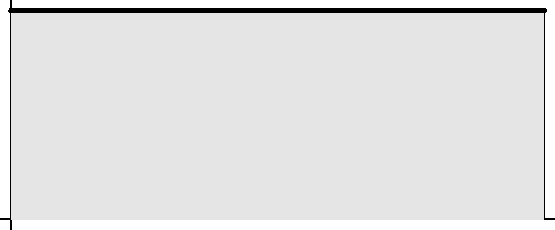
\includegraphics[width=0.22\hsize]{images/w-1}}\\
\hline
\multicolumn{4}{|c|}{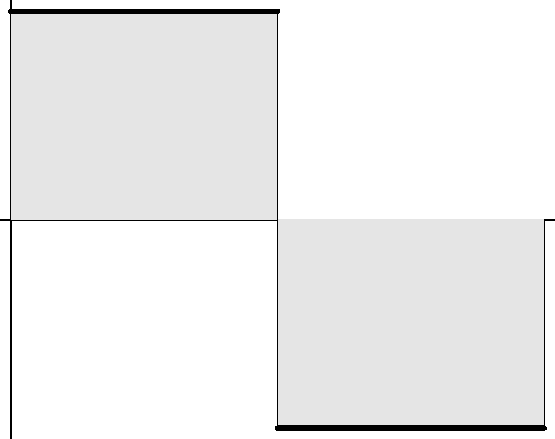
\includegraphics[width=0.22\hsize]{images/w-8}}\\
\hline
\multicolumn{2}{|c|}{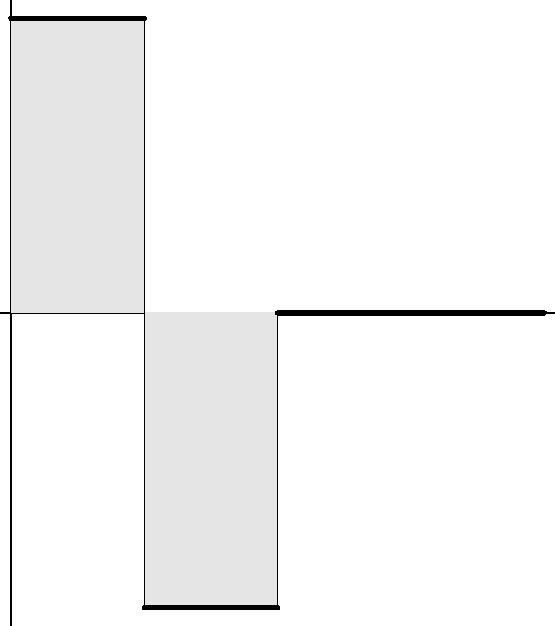
\includegraphics[width=0.22\hsize]{images/w-9}}&%
\multicolumn{2}{|c|}{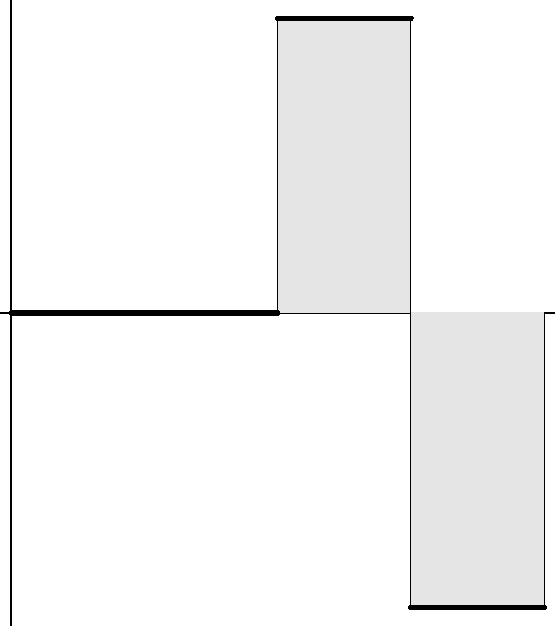
\includegraphics[width=0.22\hsize]{images/w-10}}\\
\hline
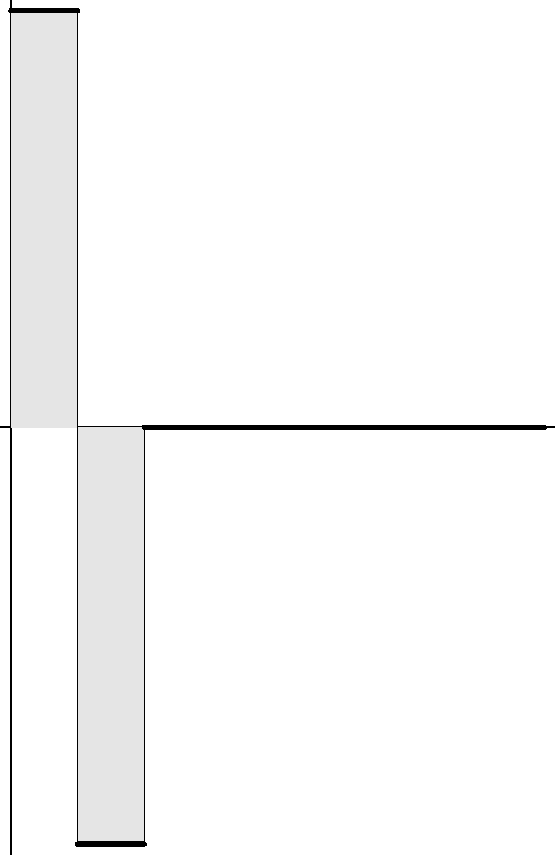
\includegraphics[width=0.22\hsize]{images/w-11}&%
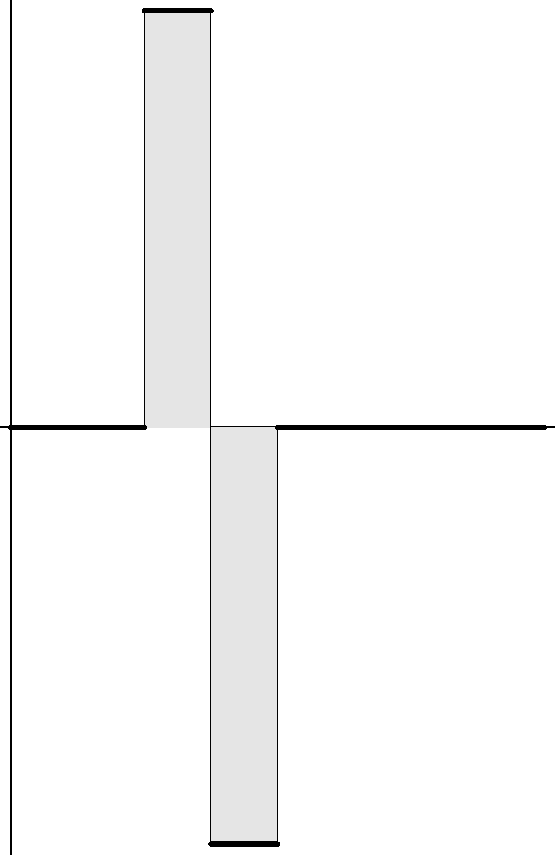
\includegraphics[width=0.22\hsize]{images/w-12}&%
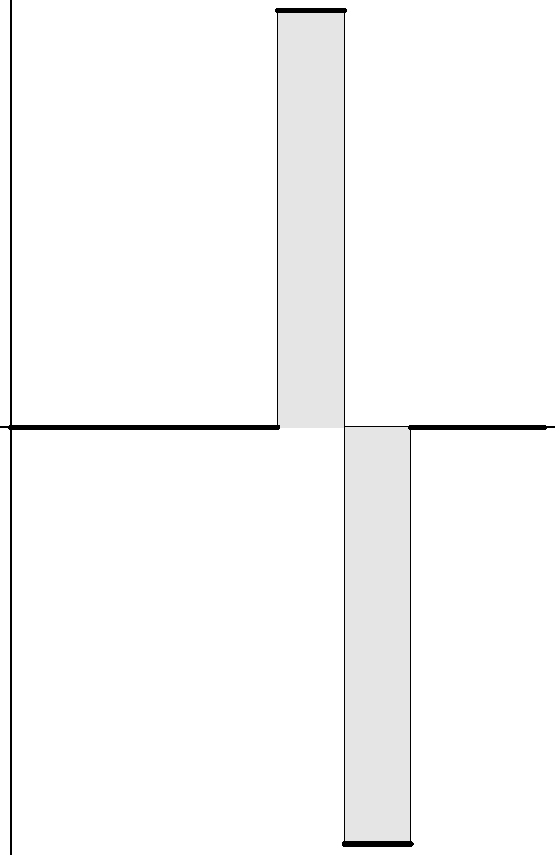
\includegraphics[width=0.22\hsize]{images/w-13}&%
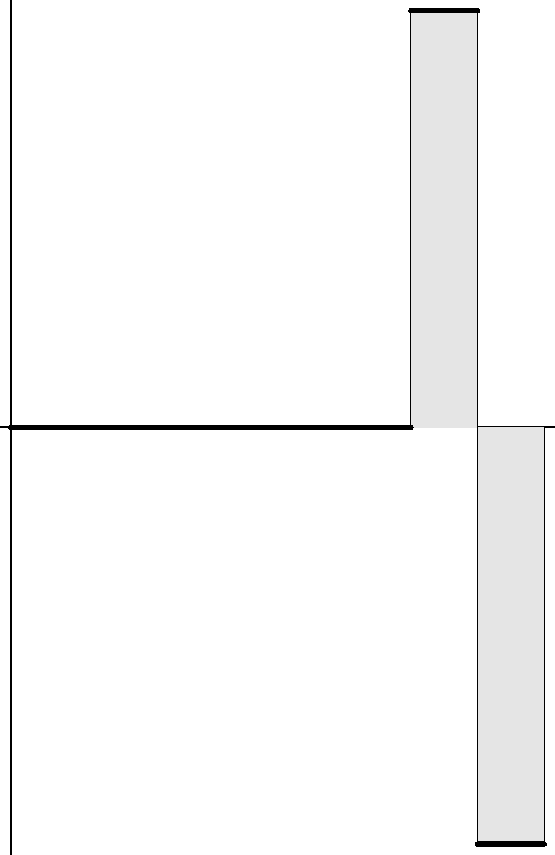
\includegraphics[width=0.22\hsize]{images/w-14}\\
\hline
\end{tabular}
\caption{Die Basisfunktionen $\psi_{i,j}$, $0\le i\le 3$ und $0\le j<2^{i-1}$.}
\end{figure}

\subsubsection{Wavelet Transformation}
Das Resultat der Analyse ist ein Vektor bestehend aus den Koeffizienten
$a_{i,j}$:
$$
{\cal W}v=\begin{pmatrix}a_{0,0}\\a_{1,0}\\a_{2,0}\\a_{2,1}\\\vdots\end{pmatrix},
$$
die sogenannte Wavelet Transformation von $v$.
Diese Transformation ist linear, f"ur zwei Signale $u$ und $v$ gilt also
\begin{align*}
{\cal W}(u+v)&={\cal W}u+{\cal W}v\\
{\cal W}(\lambda v)&=\lambda{\cal W}v
\end{align*}
Die Synthese zeigt, dass ${\cal W}$ auch umkehrbar ist, es gibt also
eine lineare Transformation ${\cal W}^{-1}$ mit
\begin{align*}
{\cal W}^{-1}{\cal W}v&=v
&
{\cal W}{\cal W}^{-1}a&=a
\end{align*}
Selbstverst"andlich kann man f"ur $\cal W$ auch eine Matrix angeben:
$$
{\cal W}
=
\frac1{\sqrt{N}}
\begin{pmatrix}
1&\dots&1&1&\dots&1&1\\
1&\dots&1&-1&\dots&-1&-1\\
\sqrt{2}&\dots&-\sqrt{2}&0&\dots&0&0\\
0&\dots&0&\sqrt{2}&\dots&-\sqrt{2}&-\sqrt{2}\\
\vdots&\ddots&\vdots&\vdots&\ddots&\vdots&\vdots\\
0&\dots&0&0&\dots&\sqrt{\frac{N}2}&-\sqrt{\frac{N}2}
\end{pmatrix}
$$
Ihre Zeilen enthalten genau die Komponenten der Vektoren
$\varphi_{0,0}$, $\psi_{i,j}$.
Die Matrix der Umkehrtransformation enth"alt dagegen die
Komponenten der Vektoren in den Spalten, also
$$
{\cal W}^{-1}
=
\frac1{\sqrt{N}}
\begin{pmatrix}
1&1&\sqrt{2}&0&\dots&0\\
\vdots&\vdots&\vdots&\vdots&\ddots&\vdots\\
1&1&-\sqrt{2}&0&\dots&0\\
1&-1&0&\sqrt{2}&\dots&0\\
\vdots&\vdots&\vdots&\vdots&\ddots&\vdots\\
1&-1&0&-\sqrt{2}&\dots&\sqrt{\frac{N}2}\\
1&-1&0&-\sqrt{2}&\dots&-\sqrt{\frac{N}2}
\end{pmatrix}
$$

\subsubsection{Anwendungen}
\begin{figure}
\begin{center}
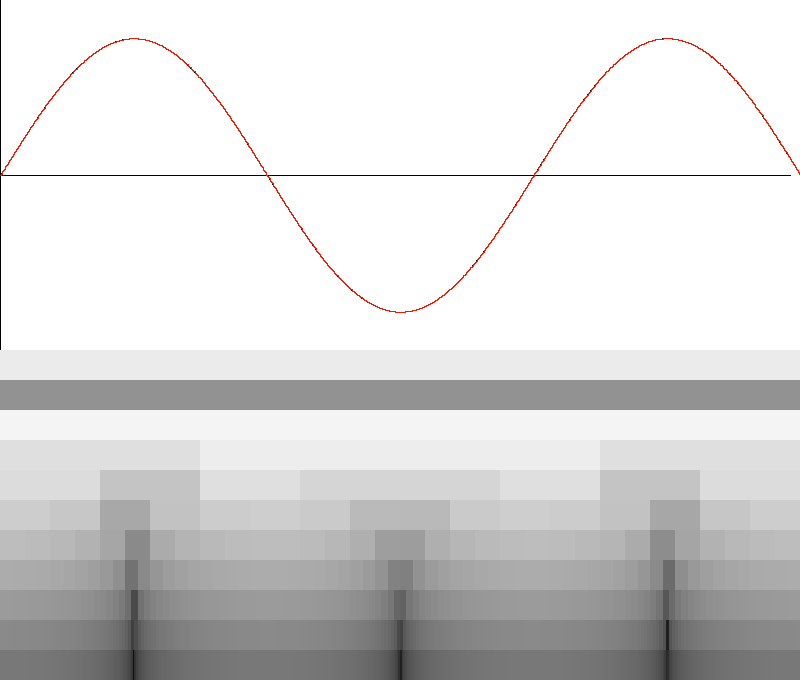
\includegraphics[width=\hsize]{graphics/wavelet-sin3}
\end{center}
\caption{Haar-Wavelet-Transformation eines Sinus-Signals. Oben das Signal,
unten die Koeffizienten $a_{i,j}$ in logarithmischer Darstellung.
Absolut kleine Koeffizienten werden dunkel dargestellt, Koeffizienten
mit grossem Absolutwert dagegen hell.\label{wavelet-sin}}
\end{figure}
\begin{figure}
\begin{center}
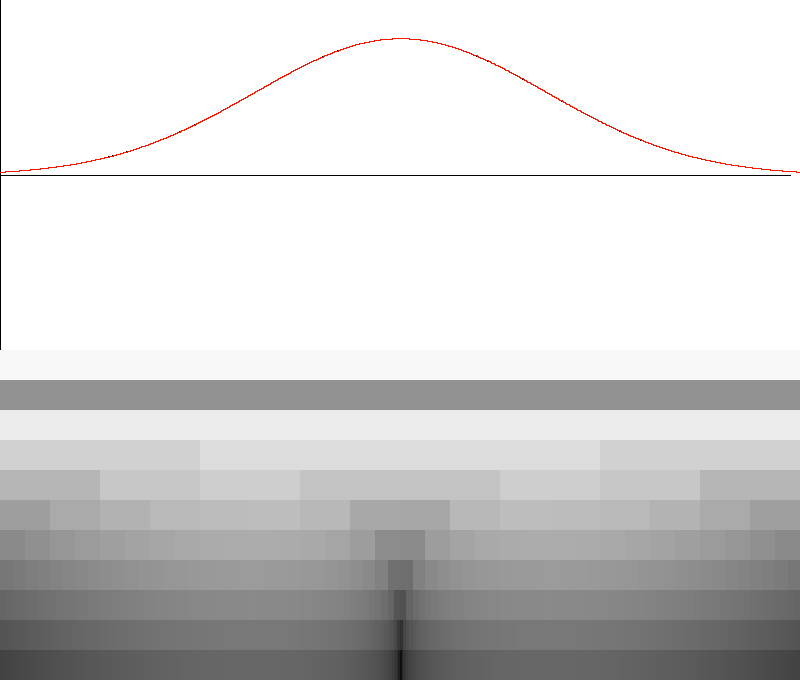
\includegraphics[width=\hsize]{graphics/wavelet-normal}
\end{center}
\caption{Haar-Wavelet-Transformation eines Gauss-Signals. Siehe 
auch Bildlegend zu Abbildung~\ref{wavelet-sin}\label{wavelet-normal}}
\end{figure}
Die Abbildungen \ref{wavelet-sin} und \ref{wavelet-normal} zeigen
die Koeffizienten $a_{i,j}$ f"ur ein Sinus-Signal und f"ur ein
ein Gauss-Signal. Da die h"oheren Koeffizienten vor allem den
Unterschied zwischen benachbarten Teilintervallen feststellen,
f"allt sofort auf, dass die h"oheren Koeffizienten in der
N"ahe der Extrema besonders klein werden.
Dagegen misst $a_{0,0}$ den Mittelwert, also das Integral des Signals.

Man kann die Wavelet Transformation zum Beispiel f"ur die Signalkomprimierung
brauchen. Nat"urliche Signale werden nicht zu schnell ansteigen, die
Koeffizienten $a_{i,j}$ f"ur $i=k-1$, welche die Zu- oder Abnahme des
Signals von Messpunkt zu Messpunkt angeben, werden also eher klein
sein. Es ist daher m"oglich, sie mit einer geringeren Anzahl von Bits
zu codieren, oder sogar ganz wegzulassen, und damit Speicherplatz zu
sparen. Nach diesem Prinzip funktioniert zum Beispiel die JPEG Komprimierung.

Nat"urlich geht durch das Weglassen von Komponenten Information verloren.
Dies wird zum Beispiel dazu verwendet, um Personen auf Bildern unkenntlich
zu machen. L"asst man alle hohen Komponenten weg, bleibt vom Signal
nur noch eine grobe Treppenfunktion "ubrig.
"Ubersetzt auf ein zweidimensionales Bild, heisst dies, dass nur noch
ein grobes Pixelraster "ubrig bleibt, auf dem eine Person nicht mehr
erkennbar ist.

Das Weglassen von hohen Komponenten kann ebenfalls mit einer Matrix
beschrieben werden:
$$
P=\begin{pmatrix}
1&\dots&0&0&\dots&0\\
\vdots&\ddots&\vdots&\vdots&\ddots&\vdots\\
0&\dots&1&0&\dots&0\\
0&\dots&0&0&\dots&0\\
\vdots&\ddots&\vdots&\vdots&\ddots&\vdots\\
0&\dots&0&0&\dots&0\\
\end{pmatrix}
$$
Der Filter, der die hochfrequenten Koeffizienten unterdr"uckt kann
also wie folgt berechnet werden:
$$
v_{\text{gefiltert}}={\cal W}^{-1}P{\cal W}v.
$$
Umgekehrt kann man die hohen Koeffizienten verst"arken. In Bildern tut
man dies zum Beispiel, um Kanten  stärker hervortreten zu lassen.
Will man die hohen Koeffizienten mit dem Faktor $\lambda$ verst"arken,
kann man dies mit dem Filter
$$
v_{\text{enhanced}}={\cal W}^{-1}(P + \lambda(I-P)){\cal W}v
$$
tun.

%
% kamera.tex
%
% (c) 2018 Prof Dr Andreas Müller, Hochschule Rapperswil
%
\documentclass[tikz]{standalone}
\usepackage{times}
\usepackage{amsmath}
\usepackage{txfonts}
\usepackage[utf8]{inputenc}
\usepackage{graphics}
\usetikzlibrary{arrows,intersections,math}
\usepackage{ifthen}
\begin{document}

\newboolean{showgrid}
\setboolean{showgrid}{false}
\def\breite{7}
\def\hoehe{4}

\begin{tikzpicture}[>=latex,thick]

% camera: w=1924px, h=1928
\node at (0,0) {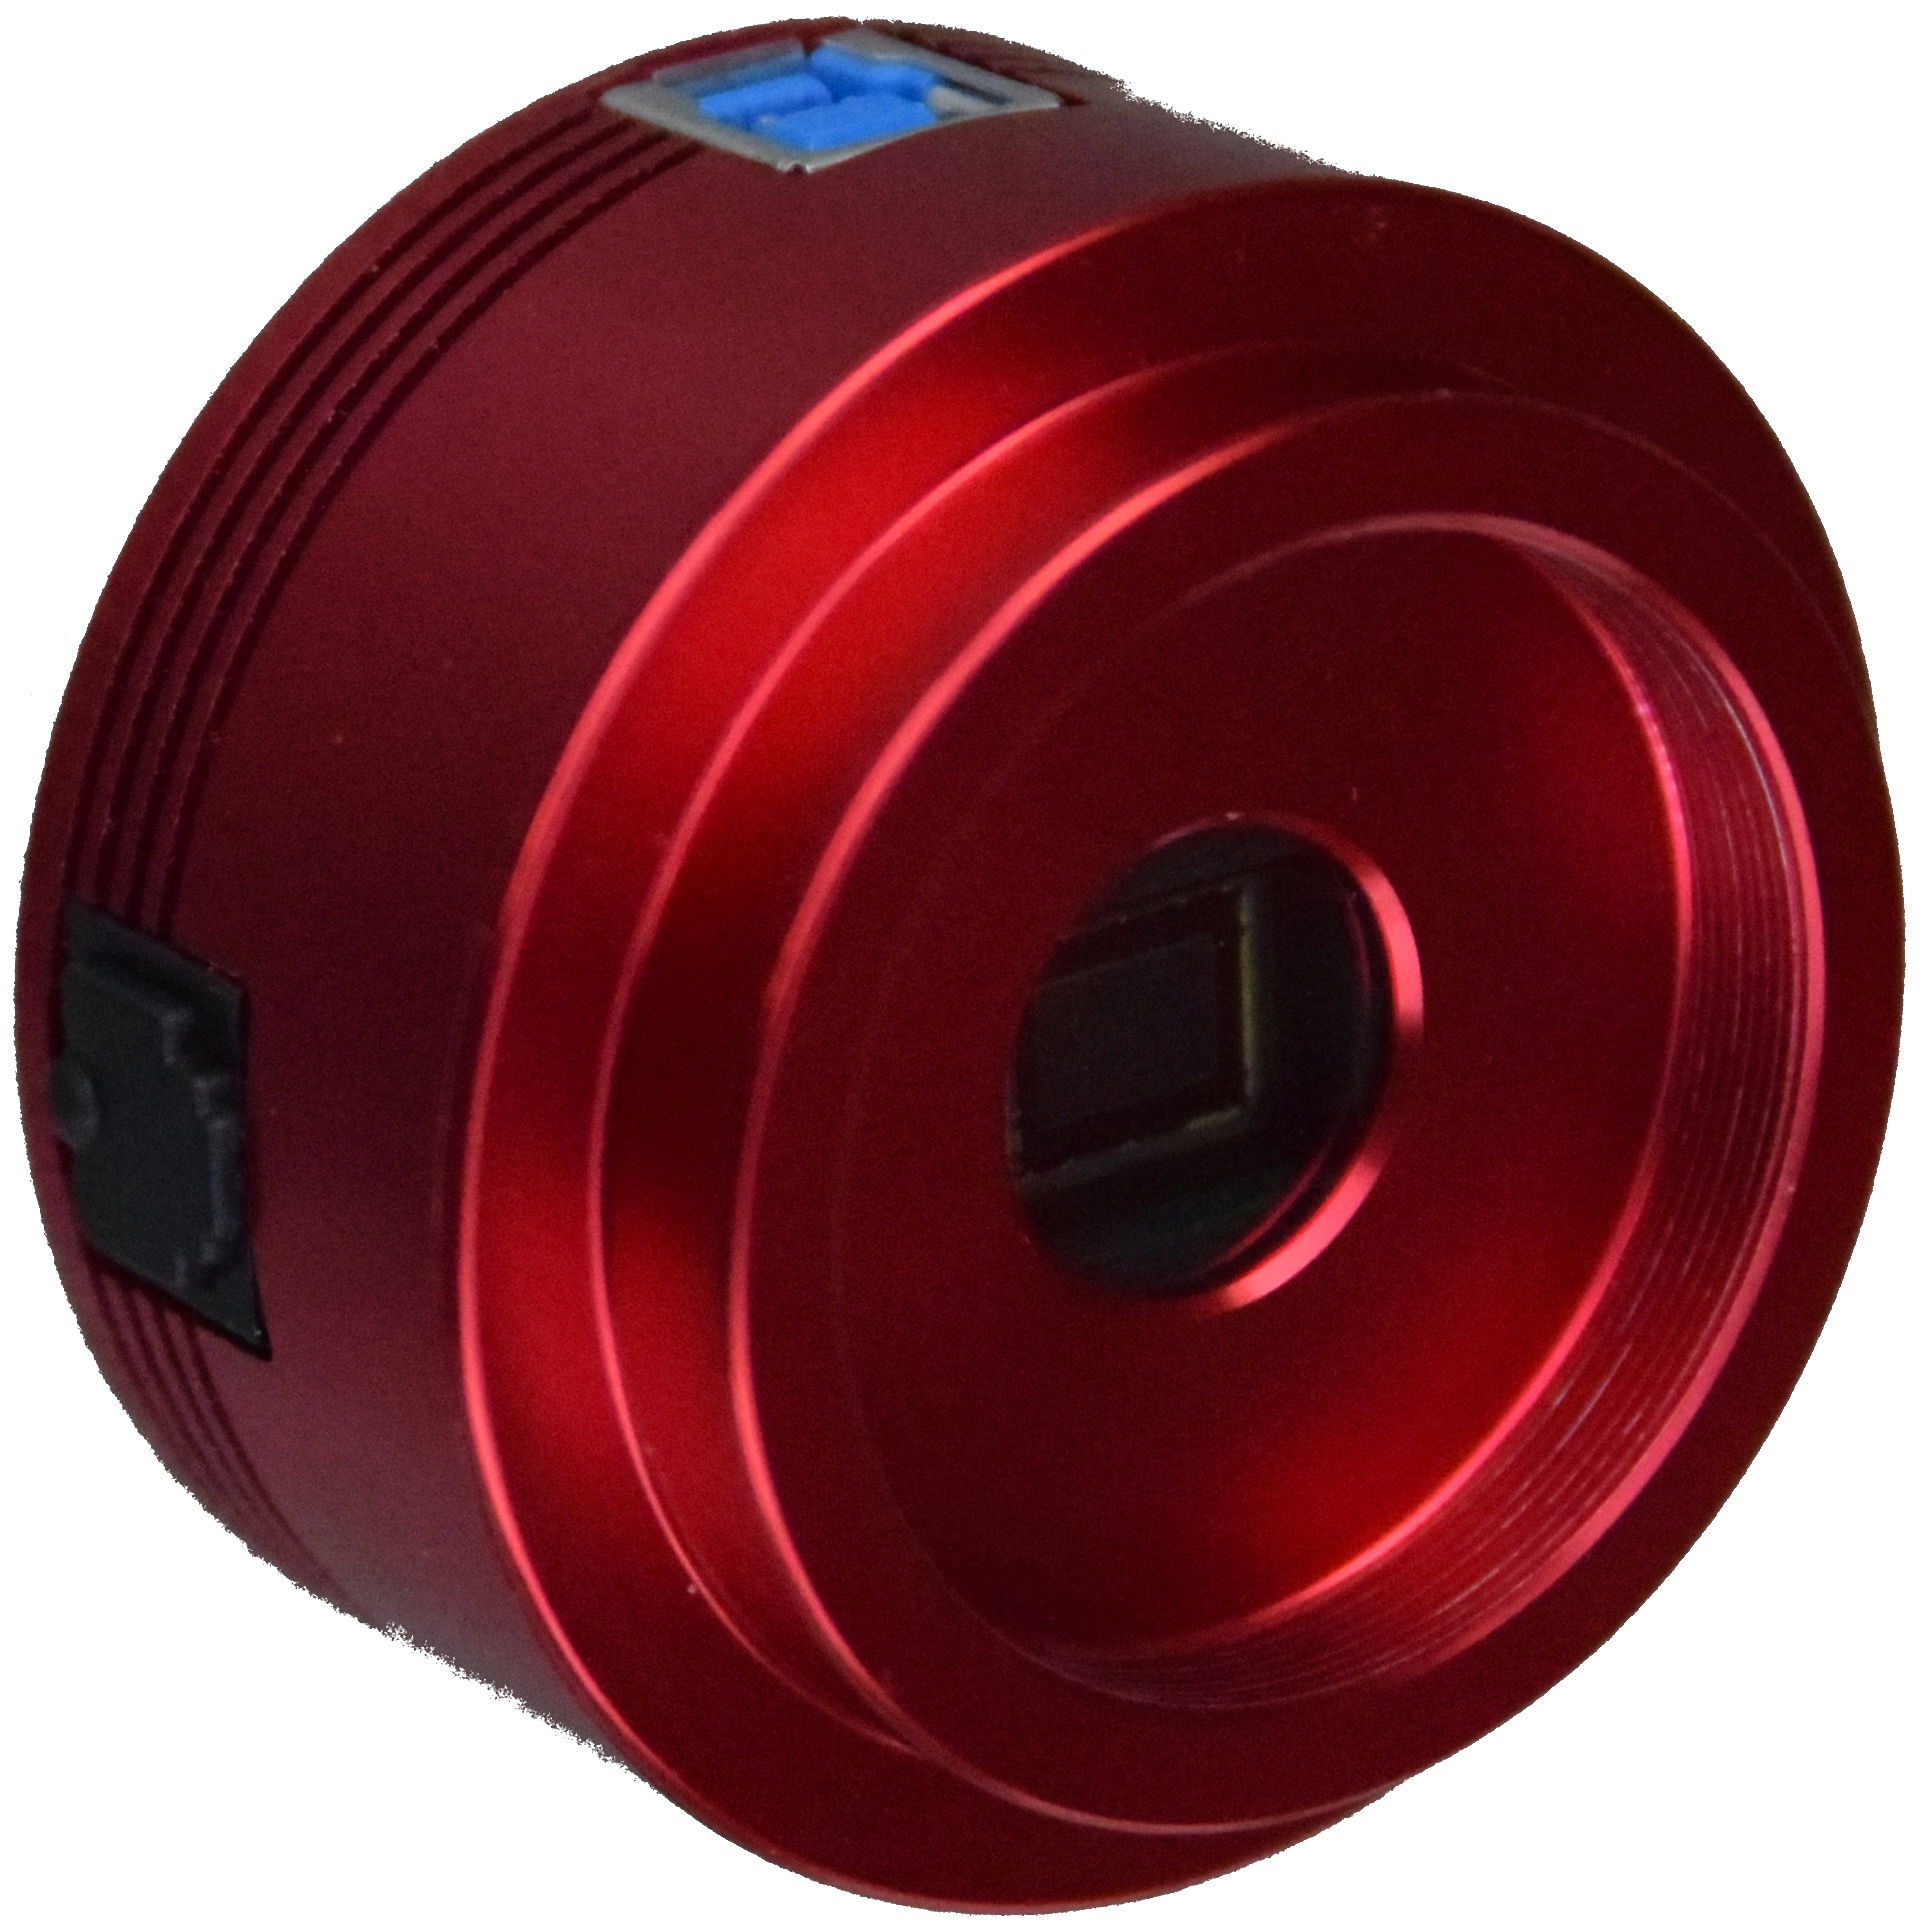
\includegraphics[width=1.924in]{camera.png}};
% objekt: w=1928px, h=1532
\node at (4.4,-1.85) {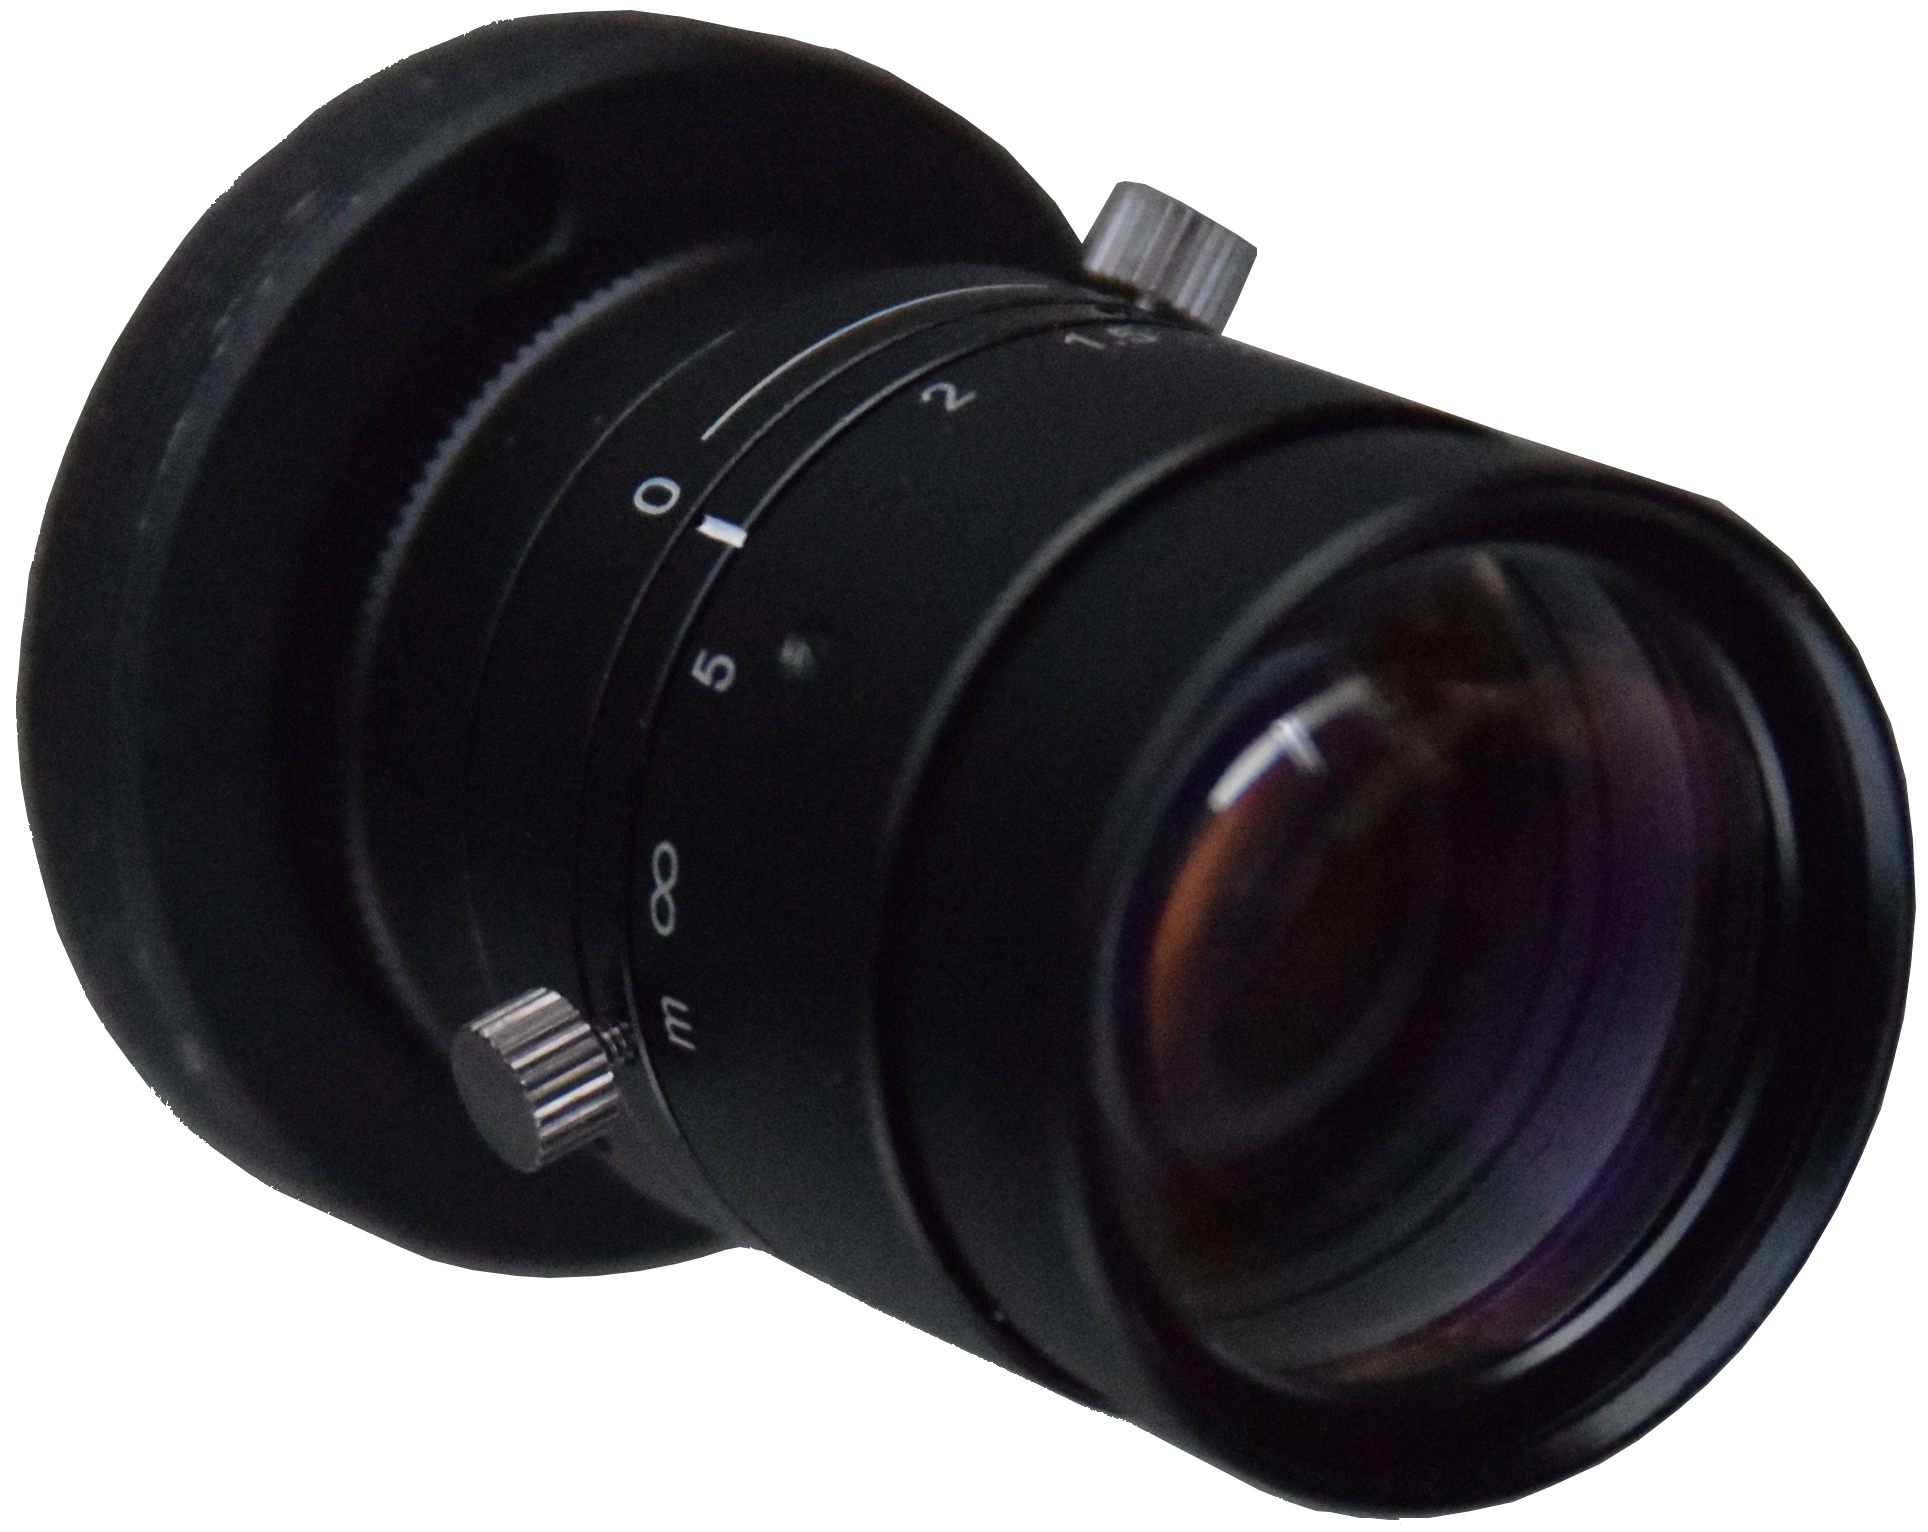
\includegraphics[width=1.85in,height=1.532in]{objektiv.png}};

% Gitter
\ifthenelse{\boolean{showgrid}}{
\draw[step=0.1,line width=0.1pt] (-\breite,-\hoehe) grid (\breite, \hoehe);
\draw[step=0.5,line width=0.4pt] (-\breite,-\hoehe) grid (\breite, \hoehe);
\draw                            (-\breite,-\hoehe) grid (\breite, \hoehe);
\fill (0,0) circle[radius=0.05];
}{}

\end{tikzpicture}

\end{document}


%
% color.tex -- RGB Farben als Beispiel eines dreidimensionalen Vektorraumes
%
% (c) 2013 Prof Dr Andreas Mueller, Hochschule Rapperswi
%
\subsection{Farben}
\subsubsection{Farben als Vektorraum}
Die Netzhaut des menschlichen Auges enth"alt zwei Arten von Rezeptoren.
Die hochemfindlichen St"abchenzellen sind vor allem f"ur gr"unes Licht
empflindlich, werden aber nur benutzt, wenn nicht ausreichend Licht
zur Verf"ugung steht.
Sie kommen vor allem bei Dunkelheit zum Einsatz, es ist mit ihnen
nicht m"oglich, Farben zu unterscheiden, daher nehmen wir in der
Nacht alles als grau war.
Auch beim Blick durch ein Teleskop kann man eine ferne Galaxie nicht
farbig sehen, da nur die St"abchenzellen empfindlich genug sind, die
uns keinen Farbeindruck liefern k"onnen. Helligkeit l"asst sich durch
eine einzige Zahl charakterisieren.

Bei Tageslicht sind die St"abchenzellen
bereits geblendet, dann kommen die Zapfen-Zellen zum Einsatz.
Sie sind viel weniger empfindlich, daf"ur gibt es sie in drei Ausf"uhrungen,
die f"ur Rot, Gr"un oder Blau empfindlich sind.
Sie erm"oglichen unser Farbensehen.
Jede Farbinformation muss sich also durch die Intensit"at wiedergeben
lassen, die die drei Arten von Zapfenzellen bestimmen k"onnen.
Die Menge aller Farben ist daher ein dreidimensionaler Vektorraum
bestehend aus Vektoren
\[
c=\begin{pmatrix}r\\g\\b\end{pmatrix}
\in\mathbb R^3,
\]
wobei $r$ das Signal der roten Zapfen, $g$ das Signal der gr"unen Zapfen
und $b$ das Signal der blauen Zapfen bezeichnet.

\subsubsection{Luminanz}
Wie hell ist eine Farbe?
Von den St"abchenzellen erhalten wir keine
Farbinformation, sondern nur Helligkeitsinformation.
Dabei bekommt der gr"une Anteil des Lichtes offenbar das
gr"osste Gewicht, weil St"abchen dort am empfindlichsten sind.
F"ur rotes und blaues Licht sind die St"abchen nicht ganz unempfindlich,
die roten und blauen Komponeten tragen also auch zum Helligkeitseindruck
bei, wenn auch in geringerem Masse.

Bei gen"ugend Licht werden die Zapfen aktiv, die Farbinformation liefern.
Trotzdem ist es uns weiterhin m"oglich, verschiedene Helligkeit
zu unterscheiden.
Offenbar ist das Gehirn in der Lage, eine Abbildung zu konsturieren,
die aus einer Farbe eine Helligkeit ableitet:
\[
L\colon \begin{pmatrix}r\\g\\b\end{pmatrix}\mapsto l.
\]
Diese Abbildung erf"ullt einige nat"urliche Bedingungen:
\begin{enumerate}
\item Wenn man zwei verschiedene Farben mischt, dann ist die Helligkeit
die Summe der Helligkeiten der einzelnen Farben:
\[
L(c_1 + c_2)=L(c_1) + L(c_2).
\]
\item Wenn man in einer Farbe alle Farbkomponenten mit dem gleichen 
Faktor verst"arkt, dann wird die Helligkeit ebenfalls um diesen Faktor
verst"arkt:
\[
L(\lambda c)=\lambda L(c).
\]
\end{enumerate}
Die Helligkeit oder {\em Luminanz} ist also eine lineare Abbildung
aus dem dreidimensionalen Farbraum in den eindimensionalen Helligkeitsraum.

Die Abbildung $L$ wird zum Beispiel ben"otigt, wenn man aus einem Farbbild
eine scharz/weiss-Bild machen m"ochte.
Nicht alle Menschen sind gleich, und so verwenden 
verschiedene technische Aufnahmesysteme
auch verschiedene lineare Abbildungen.
\begin{align}
L&=0.2126 r+0.7152 g + 0.0722 b\tag{ITU-r}
\\
L&=0.299 r + 0.587 g + 0.114 b\tag{CCIR601}
\\
L&=0.33 r + 0.5 g + 0.16 b\notag
\\
L&=0.375 r + 0.5 g + 0.125 b\notag
\end{align}
Die letzten zwei Formeln stimmen nicht besonders gut mit der tats"achlichen
Empfindlichkeitsverteilung der St"abchenzellen "uberrein, aber sie lassen
sich extrem rasch berechnen, was f"ur die Hersteller von Video-Kameras 
interessant ist.

Wir weisen darauf hin, dass die oben aufgelisteten Luminanz-Funktionen
alle die Eigenschaft haben, dass die Summe der Koeffizienten $1$ ist.
Wir verwenden das als Definition:
\begin{definition} Eine {\em Luminanz-Funktion} $L$ ist eine lineare Abbildung
des Farbraums in den Helligkeitsraum der Form
\[
L(c)=\rho \cdot r + \gamma \cdot g + \beta \cdot b
\]
mit den Eigenschaften
\begin{enumerate}
\item alle Koeffizienten $\rho$, $\gamma$ und $\beta$ sind positiv,
\item die Summe der Koeffizienten ist $1$.
\end{enumerate}
\end{definition}
Die Luminanz ist ein gewichtetes Mittel der Farbkomponenten.

\subsubsection{Farbs"attigung}
In diesem Abschnitt gehen wir von einer festen Luminanzfunktion aus.
Die Menge der Farben, die gleich hell sind wie eine vorgegebene Farbe $c_1$,
ist 
\[
\{ c\in\mathbb R^3\,|\, L(c)=L(c_1)\}.
\]
Diese Menge ist eine Ebene im Farbraum.

Gibt es einen Grauton $c_0$, welcher gleich hell ist wie $c_1$?
Damit wir diese Farbe als Grauton wahrnehmen, m"ussen alle drei Farbkomponenten
gleich sein, wir schreiben f"ur diese drei identischen Komponenten $x$,
bekommen also
\[
c_0=\begin{pmatrix}x\\x\\x\end{pmatrix}.
\]
Die zugeh"orige Luminanz ist
\[
L(c_0)=\rho\cdot x + \gamma\cdot x + \beta \cdot x=
(\rho + \gamma +\beta)\cdot x=x
\]
Der zu einer Farbe $c$ geh"orige graue Farbe ist also
\[
\begin{pmatrix}L(c)\\L(c)\\L(c)\end{pmatrix}
=
L(c)\begin{pmatrix}1\\1\\1\end{pmatrix}
\]
Wir schreiben f"ur den Vektor aus lauter Einsen in Zukunft $w$ (f"ur weiss):
\[
w=\begin{pmatrix}1\\1\\1\end{pmatrix}, \qquad L(w)=1.
\]
Wir k"onnen also eine Farbe $c_1$ immer in zwei Komponenten zerlegen,
eine monochrome Komponente und eine Komponente parallel zur Ebene
$\{ c\,|\, L(c)=L(c_1)\}$:
\[
c_1 = \underbrace{L(c_1)w}_{\text{Helligkeit}} + \underbrace{(c_1 - L(c_1)w)}_{\text{Farbe}}.
\]
Die Farbinformation steckt ausschliesslich im zweiten Term, der erste
Term gibt die Helligkeit wieder.
Damit bekommen wir eine M"oglichkeit, bei gleichbleibender Helligkeit
die Intenit"at der Farben zu ver"andern. Schreiben wir
\[
c(t)=L(c_1)w+t(c_1-L(w))w,
\]
dann liefert der Wert $t=0$ eine Farbe, die ein Vielfaches von $w$ ist, also
ein Grauwert. F"ur $t=1$ erhalten wir die urspr"ungliche Farbe zur"uck.
Die Zwischenwerte $0 < t < 1$ liefern Farben mit zunehmender Farbintensit"at,
oder wie man sagt, {\em Farbs"attigung}. 
Wir sind sogar in der Lage, die Farbe noch intensiver zu machen, indem
wir $t>1$ w"ahlen.
In der Abbildung~\ref{color:saettigung}
ist ein Bild mit verschiedenen Werten von $t$ gezeigt.
\begin{figure}
\begin{center}
\begin{tabular}{cccc}
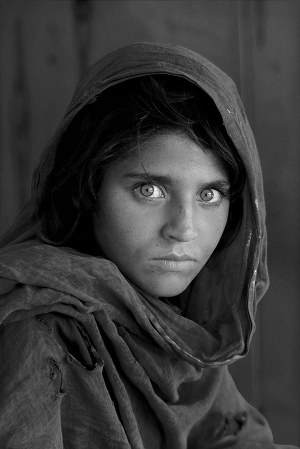
\includegraphics[width=0.22\hsize]{graphics/saettigung0.jpg}&%
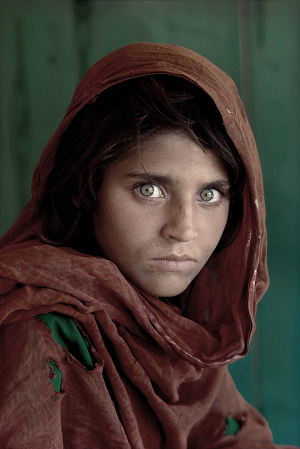
\includegraphics[width=0.22\hsize]{graphics/saettigunghalb.jpg}&%
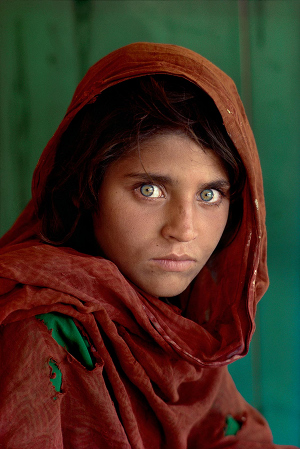
\includegraphics[width=0.22\hsize]{graphics/saettigung1.jpg}&%
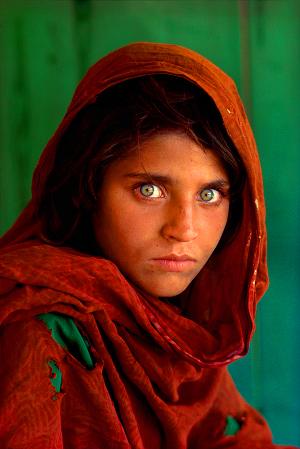
\includegraphics[width=0.22\hsize]{graphics/saettigung2.jpg}\\
$t=0$&$t=\frac12$&$t=1$&$t=2$
\end{tabular}
\end{center}
\caption{S"attigung f"ur verschiedene Werte von $t$
\label{color:saettigung}}
\end{figure}

\subsubsection{Farbton}
Die Farben gleicher Helligkeit bilden eine Ebene. In der Ebene gibt es
den ausgezeichneten Punkt $L(c_1)w$, der dem gleich hellen Grauton
entspricht. Wir nennen diesen Punkt auch den {\tt Weisspunkt}.
Je weiter entfernt ein Punkt $c$ in der Ebene von diesem
Punkt ist, desto intensiver die Farben, desto gr"osser die Farbs"attigung.

Ein Punkt in der Ebene $H=\{c\,|\, L(c)=L(c_1)\}$ ist aber durch
den Abstand vom Weisspunkt alleine nicht bestimmt. Durch Wahl einer 
geeigneten Null-Richtung k"onnen wir in der Ebene $H$ ein
Polarkoordinaten-System w"ahlen. Der Winkel entspricht dabei dem
Farbton.
Die Menge aller vom menschlichen Auge wahrnehmbaren k"onnen daher
auf einem Kreis angeordnet werden, dem Farbkreis.

Damit haben wir ein alternatives Koordinatensystem f"ur den Farbraum
konstruiert mit den drei Koordinaten
\begin{center}
\begin{tabular}{l|l}
\hline
Hue&Farbton, Farbwinkel\\
Saturation&Farbs"attigung\\
Brightness&Luminanz\\
\hline
\end{tabular}
\end{center}
Der Vorteil dieses Koordinatensystems gegen"uber dem RGB-System ist,
dass sich Bildverarbeitungsoperationen wie ``Heller'' oder ``mehr Farbe''
darin leichter beschreiben lassen.

%
% qam.tex -- Quadratur-Amplituden-Modulation mit Matrizen und Vektorgeometrie
%
% (c) 2020 Prof Dr Andreas Müller, Hochschule Rapperswil
%
\section{Quadratur-Amplituden-Modulation
\label{section:quadratur-amplituden-modulation}}
\rhead{Quadratur-Amplituden-Modulation}
Um ein zeitabhängiges Signal drahtlos zu übertragen, muss es auf
ein hochfrequentes Trägersignal aufmoduliert werden.
Wie macht man das und wie kann man das ursprüngliche Signal
wiedergewinnen?
Eine besonders flexible Methode, die sogenannte
Quadratur-Amplituden-Modu\-lation, lässt sich mit Hilfe von Vektorgeometrie
und Drehmatrizen besonders leicht verstehen.


%
% amplitudenmodulation.tex
%
% (c) 2020 Prof Dr Andreas Müller, Hochschule Rapperswil
%
\subsection{Amplitudenmodulation
\label{subsection:amplitudenmodulation}}
Die Technik der Amplitudenmodulation geht auf die Anfangszeit des
Radios zurück.
Um ein zeitabhängiges Audio-Signal $I(t)$ mit Frequenzen von typischwerweise
wenigen hundert Herz oder wenigen Kilohertz drahtlos zu übertragen,
verändert man die Amplitude eines Trägersignals von mehreren hundert
Kilohertz oder mehr und leitet es zu einer Antenne.
Diese strahlt dann eine entsprechend oszillierendes elektromagnetisches
Feld ab, welches von einem Empfänger aufgefangen und wieder hörbar gemacht
werden kann.

\begin{figure}
\centering
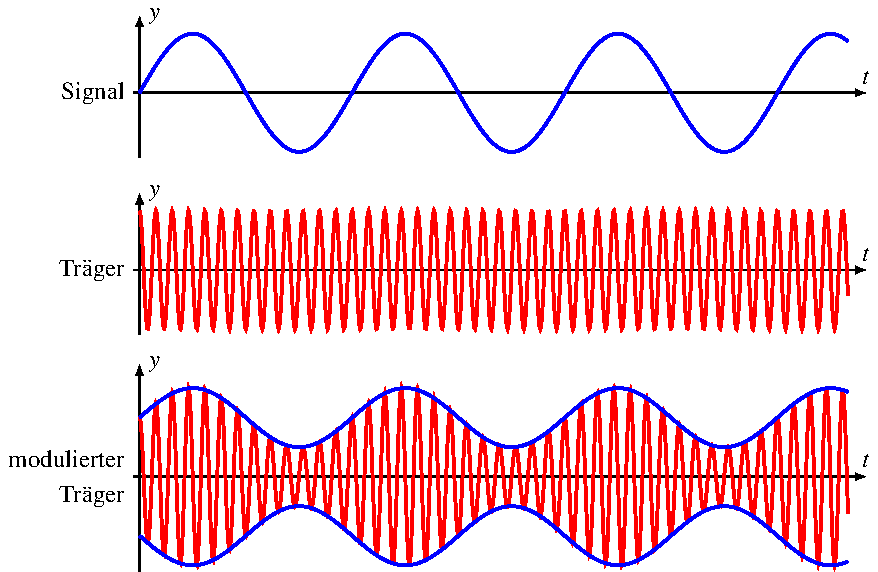
\includegraphics{applications/qam/am.pdf}
\caption{Amplitudenmodulation eines Signals $I(t)$ auf eine
Trägerfrequenz $\cos\omega t$.
Die Amplitude des Trägers wird im Takt des Signals verändert.
\label{figure:qam:am}}
\end{figure}

In Abbildung~\ref{figure:qam:am} wird die Amplitude des Träger
$\cos\omega t$ mit der Kreisfrequenz $\omega$ wird im Takt des
Signals verändert,
konkret wird der Träger mit $1+I(t)$ multipliziert,
das übermittelte Signal ist also
\begin{equation}
(1+I(t)) \cos\omega t.
\end{equation}
Ein so moduliertes Signal ist besonders leicht zu demodulieren.
Es reicht, das Signal gleichzurichten und verbleibenden Reste
der Trägerfrequenz sowie die konstente Komponten auszufiltern.
Ein
\begin{figure}
\centering
\begin{tikzpicture}
\node at (0,0) {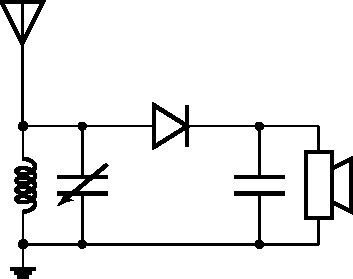
\includegraphics{applications/qam/detektor.pdf}};
\node at (8,0) {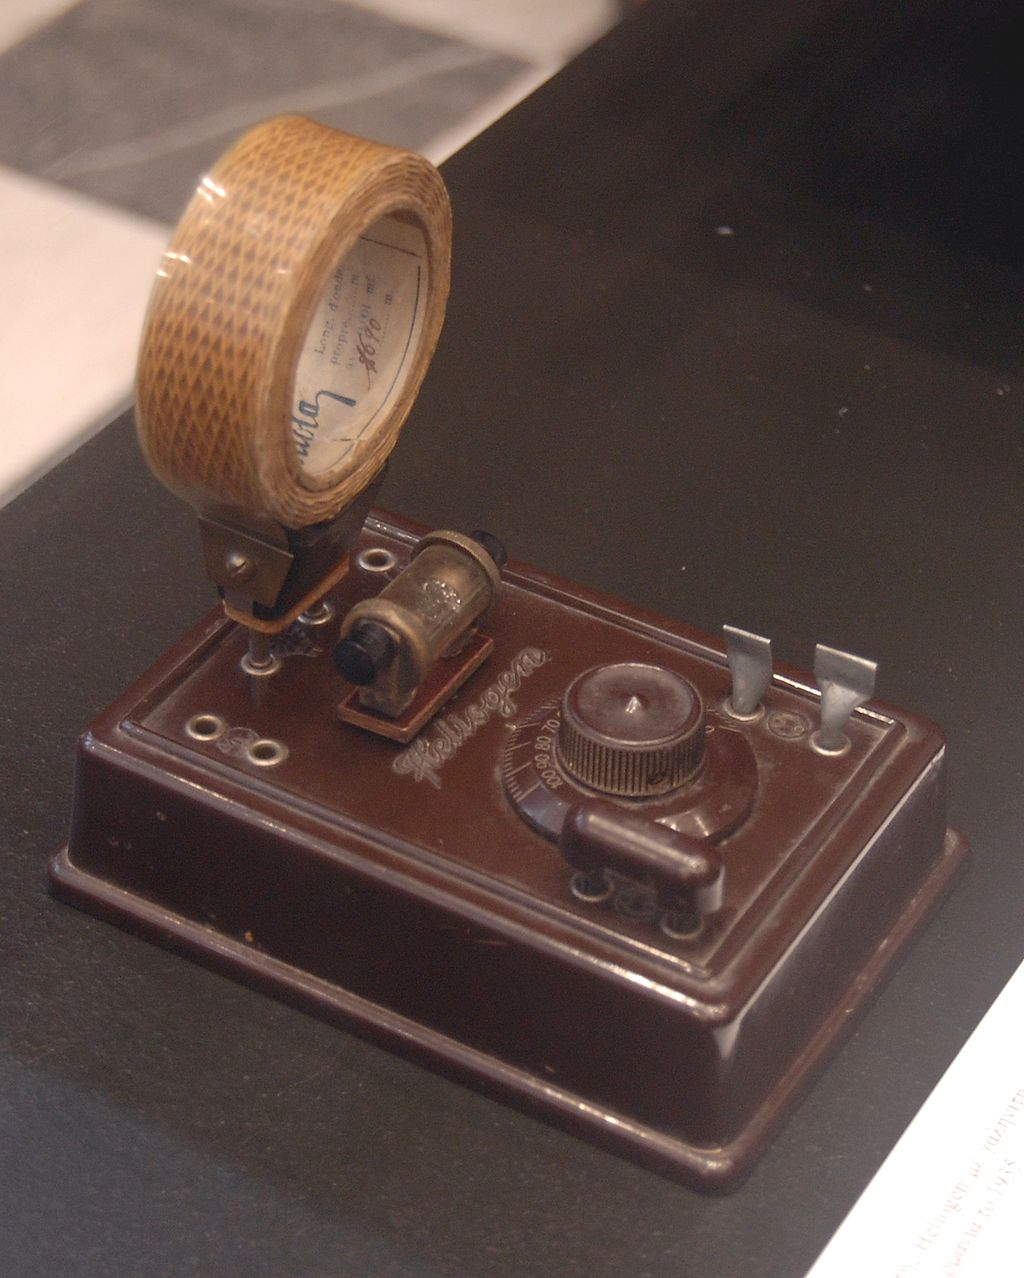
\includegraphics[width=6cm]{applications/qam/detektor.jpg}};
\end{tikzpicture}
\caption{Ein Detektorradio besteht aus einem einstellbaren
Schwingkreis zur Auswahl der Trägerfrequenz, einer Diode zur
Gleichrichtung und einem Kondensator zur Filterung der Überreste
des Trägers.
Bei starken Sendern kann das niederfrequente Tonsignal ohne
Verstärkung mit einem Kopfhörer abgehört werden.
\label{figure:qam:detektor}}
\end{figure}
Die konstante Komponente (der Summand $1$) ist nicht wirklich
interessant und dient nur einer leichter verständlichen Darstellung
in Abbildung~\ref{figure:qam:am}, wir werden sie in Zukunft 
ignorieren und nur noch das modulierte Signal $I(t)\cos\omega t$
betrachten.

Mit dieser Methode kann man zu jeder Zeit $t$ einen einzelnen
Wert $I(t)$ übermitteln.
Für die Praxis ist das schon bei Audiosignalen oft ungenügend, man
möchte doch mindestens die beiden Stereokanäle eines qualitativ
hochwertigen Signals übertragen können.

Die zweite Schwierigkeit ist die Frage, warum wir $\cos\omega t$
dem ebenfalls möglichen Träger $\sin\omega t$ vorziehen sollen.
Die beiden unterscheiden sich nur um eine Phasenverschiebung
von $90^\circ$, die für die oben beschriebene Modulation und
Demodulation bedeutungslos ist.







%
% zweidimensionale.tex
%
% (c) 2020 Prof Dr Andreas Müller, Hochschule Rapperswil
%
\subsection{Zweidimensionale Signale
\label{subsection:qam:zweidimensional}}
Wir suchen also nach einem Verfahren, mit welchem wir nicht nur
ein einzelnes zeitabhängiges Signal $I(t)$ übertragen können, sondern
auch noch ein zweites Signal, welches wir mehr oder weniger aus
historischen Gründen $Q(t)$ nennen wollen\footnote{Das Signal $I(t)$
heisst auch die In-phase-Komponente und $Q(t)$ Quadratur-Komponente}.
Man kann sich die beiden Signale zum Beispiel also die beiden
Stereokanäle eines Audiosignals vorstellen.
Wir stellen uns die beiden Komponenten als untrennbar zusammengehörig
vor, es ist daher sinnvoll, sie als zweidimensionalen Vektor
\[
\vec{v}(t)
=
\begin{pmatrix}I(t)\\Q(t)\end{pmatrix}
\]
zu schreiben.
Dieser Vektor beschreibt zu jeder Zeit $t$ einen Punkt in der
$I$-$Q$-Ebene.
Zu verschiedenen Zeiten beschreibt $\vec{v}(t)$ eine Kurve
in der Ebene.
Mit einem Oszilloskop im X-Y-Modus kann man den Vektor
sichtbar machen.
Zum Beispiel führt das Signal
\begin{equation}
I(t) = \cos t,\quad
Q(t) = \sin 3t
\qquad
\Rightarrow
\qquad
\vec{v}(t)
=
\begin{pmatrix}
\cos t\\
\sin 3t
\end{pmatrix}
\label{eqn:qam:liss1}
\end{equation}
auf die in Abbildung~\ref{figure:qam:lissajous} dargestellte Kurve.
\begin{figure}
\centering
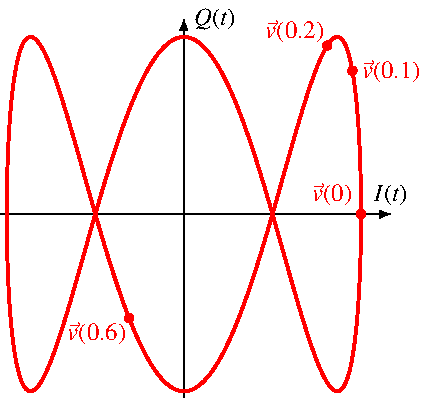
\includegraphics[width=0.48\hsize]{applications/qam/images/lissajous.pdf}
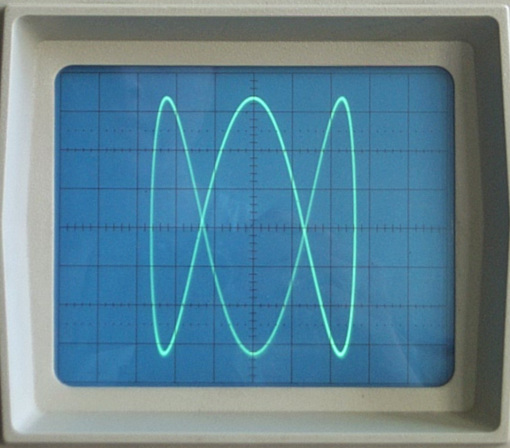
\includegraphics[width=0.48\hsize]{applications/qam/images/lissajous.jpg}
\caption{Lissajous-Figur des zweidimensionalen Signals
\eqref{eqn:qam:liss1} kann auf einem Oszilloskop im X-Y-Modus
sichtbar gemacht werden.
\label{figure:qam:lissajous}}
\end{figure}
Solche Kurven sind bekannt als Lissajous-Figuren.
Mit komplizierteren Funktion $I(t)$ und $Q(t)$ kann fast jede
Linienzeichnung auf den Schirm des Oszilloskops gezaubert werden,
wie zum Beispiel auch die Internet ``Kunstform'' der Oscilloscope
Music (\url{https://www.youtube.com/watch?v=qnL40CbuodU}) zeigt.
In Abbildung~\ref{figure:qam:pilze} werden zum Beispiel Pilze und
ein Schmetterling mit zwei geeigneten Funktionen $I(t)$ und $Q(t)$
gezeichnet.

\begin{figure}
\centering
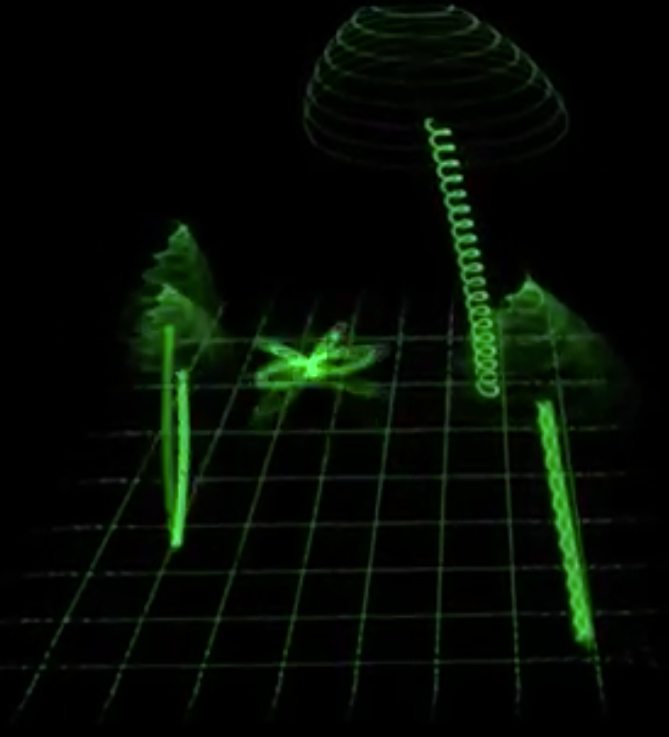
\includegraphics[width=0.5\hsize]{applications/qam/images/pilze.png}
\caption{Pilze und ein Schmetterling gezeichnet von zwei Signalen
$I(t)$ und $Q(t)$ aus dem Video \url{https://youtu.be/rtR63-ecUNo}
\label{figure:qam:pilze}}
\end{figure}




%
% modulation.tex
%
% (c) 2020 Prof Dr Andreas Müller, Hochschule Rapperswil
%
\subsection{Modulation zweidimensionaler Signale
\label{subsection:modulation}}
Wir streben jetzt an, ein zweidimensionales Signal
\[
\vec{v}(t)
=
\begin{pmatrix}I(t)\\Q(t)\end{pmatrix}
\]
drahtlos zu übertragen und müssen zu diesem Zweck ein geeignetes
Modulationsverfahren finden.

\begin{figure}
\centering
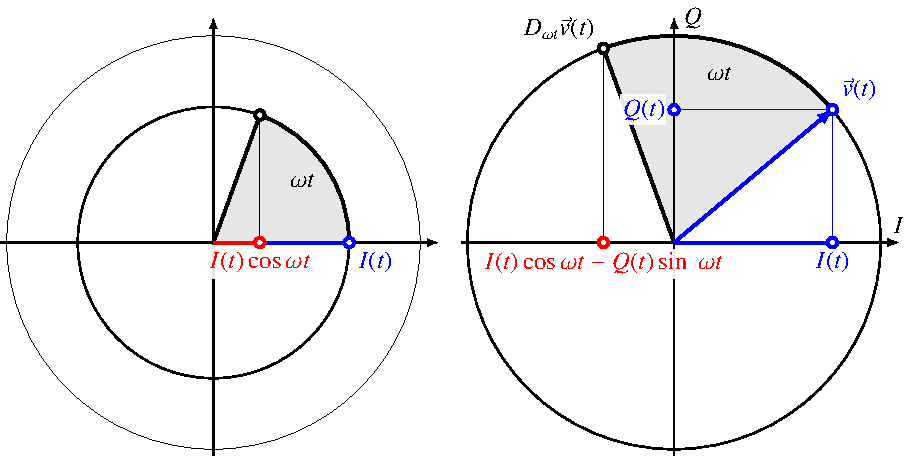
\includegraphics{applications/qam/images/icos.pdf}
\caption{Modulation des Signals $I(t)$ als Drehung um den Winkel $\omega t$
auf einem Kreis mit Radius $I(t)$.
\label{qam:figure:icos}}
\end{figure}
Mit nur dem einen Signal $I(t)$ haben wir $I(t)\cos\omega t$ als moduliertes
Signal gewählt.
Geometrisch können wir das auf einem Kreis mit Radius $I(t)$ als Drehung
um den Winkel $\omega t$ mit anschliessender Projektion auf die horizontale
Achse verstehen (Abbildung~\ref{qam:figure:icos} links).

Es ist daher naheliegend, für die Modulation des zweidimensionalen Signals
ebenfalls eine Drehung um den Winkel $\omega t$ zu verwenden.
Der Vektor $\vec{v}(t)$ wird in der $I$-$Q$-Ebene gedreht wie in
Abbildung~\ref{qam:figure:icos} rechts gezeigt.
Dazu kann eine Drehmatrix $D_{\omega t}$ verwendet werden.
Wir berechnen
\begin{equation}
D_{\omega t}
\vec{v}(t)
=
\begin{pmatrix}
\cos\omega t & -\sin\omega t\\
\sin\omega t &\phantom{-}\cos\omega t
\end{pmatrix}
\begin{pmatrix}I(t)\\Q(t)\end{pmatrix}
=
\begin{pmatrix}
I(t)\cos\omega t - Q(t) \sin\omega t\\
I(t)\sin\omega t + Q(t) \cos\omega t
\end{pmatrix}
=
\begin{pmatrix}
s(t)\\c(t)
\end{pmatrix}
\label{qam:eqn:modulation}
\end{equation}
Das zweite Signal $Q(t)$ modulieren wir also statt mit $\cos\omega t$ 
mit der Funktion $-\sin\omega t$.
Natürlich können wir aus den beiden Funktionen $I(t)\cos\omega t$ und
$-Q(t)\sin\omega t$ auch die Funktionen $I(t)$ und $Q(t)$ zurückgewinnen,
das reicht aber nicht.
Dazu brauchen wir nämlich $I(t)\cos\omega t$ und $-Q(t)\sin\omega t$
unabhängig voneinander, wir brauchen also zwei unabhängig Übertragungskanäle
für die beiden Signale, was wir vermeiden wollen.

\begin{figure}
\centering
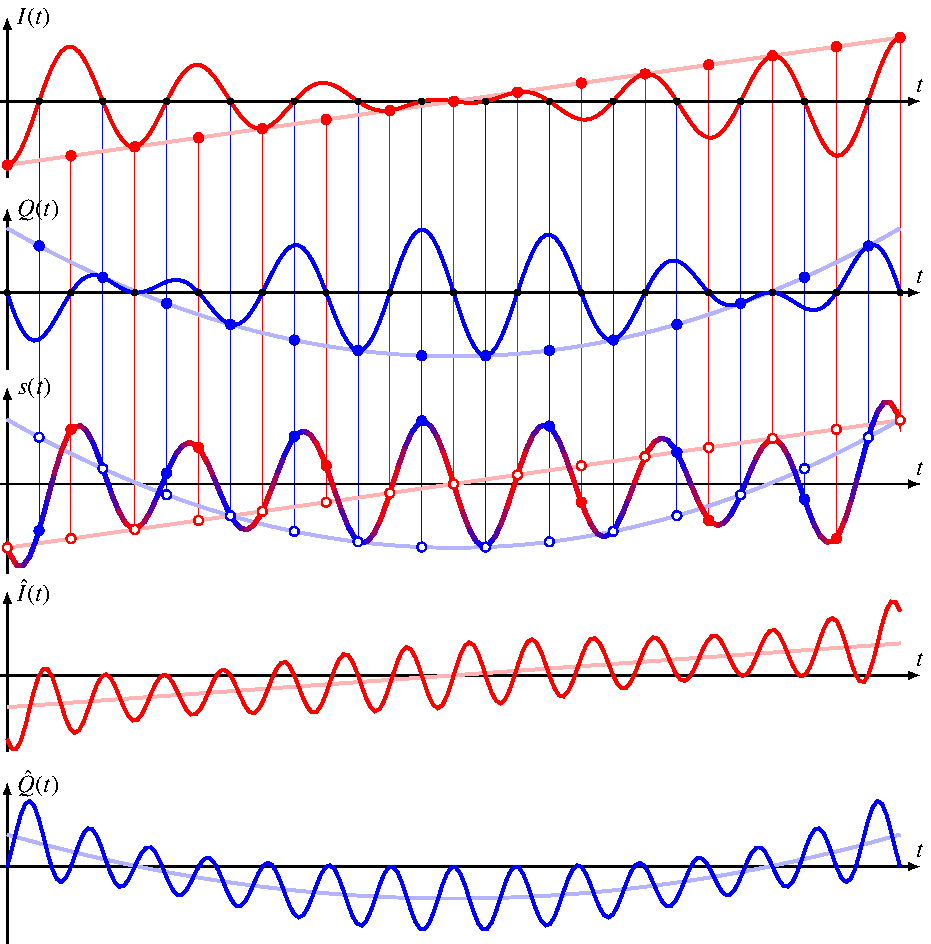
\includegraphics{applications/qam/images/sep.pdf}
\caption{Rekonstruktion der Signale $I(t)$ und $Q(t)$ (oberste zwei Graphen)
aus der Summe $s(t) = I(t)\cos\omega t - Q(t)\sin\omega t$ (Mitte).
Die Nullstellen von $\cos\omega t$ sind durch feine blaue Linien 
dargestellt, die Nullstellen von $\sin\omega t$ durch feine rote Linien.
Der Graph von $s(t)$ ist jeweils mit der Farbe eingefärbt, die den
dominanten Beitrag repräsentiert.
Blaue Segmente im Graphen von $s(t)$ bedeuten, dass vor allem der Wert
von $Q(t)$ zum Wert beiträgt, dies geschieht in der Umgebung von
Nullstellen von $\cos\omega t$, in den roten Segmenten ist es der Wert von
$I(t)$, welcher dominiert während $\sin\omega t$ eine Nullstelle durchläuft.
Fette Punkte auf dem Graphen von $s(t)$ markieren Punkte bei den
genannten Nullstellen.
Die leeren Punkte sind Werte von $s(t)$, die um das Vorzeichen des
Trägeres korrigiert wurden, sie liegen genau auf dem Graphen der
ursprünglichen Signale $I(t)$ und $Q(t)$.
Die untersten zwei Graphen zeigen die rekonstruierten Signale
$\hat{I}(t)=s(t) \cos\omega t$ und $\hat{Q}(t) = -s(t) \sin\omega t$, 
welche in Abschnitt~\ref{subsection:demodulation} erklärt werden.
\label{figure:qam:sep}}
\end{figure}

Einzelne Werte der Funktionen $I(t)$ und $Q(t)$ können aber aus der Summe
\[
s(t)
=
I(t)\cos\omega t - Q(t)\sin\omega t
\]
rekonstruiert werden.
An den Stellen $t = k\pi/\omega$ für $k\in\mathbb Z$ verschwindet
der Faktor $\sin\omega t$,
so dass an diesen Stellen der zweite Summand in $s(t)$ wegfällt.
Ebenso wird der erste Summand an den Stellen
$t = (k+\frac12)\pi/\omega$ verschwinden.
Dieser Sachverhalt ist in Abbildung~\ref{figure:qam:sep} dargestellt.
Es ist also
\[
s\biggl(k\cdot \frac{\pi}{2\omega}\biggr)
=
\begin{cases}
I(k\cdot \frac{\pi}{2\omega})\cdot(-1)^{\frac{k}2}
&\qquad \text{$k$ gerade,}\\[5pt]
Q(k\cdot \frac{\pi}{2\omega})\cdot(-1)^{\frac{k-1}2}
&\qquad \text{$k$ ungerade.}
\end{cases}
\]
Zu Zeitpunkten, die Vielfache von $\pi/2\omega$ sind, kann man also aus
$s(t)$ die Werte von $I(t)$ und $Q(t)$ ablesen.
Tatsächlich lernt man im Fach {\em Signale und Systeme}, dass man daraus
die Funktionen $I(t)$ und $Q(t)$ rekonstruieren kann, wenn sie keine
Frequenzkomponenten grösser als die Trägerfrequenz haben.
Die Summe $s(t)$ ist also etwas, was man potentiell drahtlos übermitteln
kann, und woraus man die Komponenten $I(t)$ und $Q(t)$ zurückgewinnen kann.
Man nennt dieses Modulationsverfahren {\em Quadratur-Amplituden-Modulation}.

Da wir über das nötige signaltheoretische Wissen noch nicht verfügen,
müssen wir eine alternative, geometrische Methode suchen, wie wir
aus $s(t)$ die Komponenten $I(t)$ und $Q(t)$ wiedergewinnen können.
Das modulierte Signal $s(t)$ ist also nichts anderes als eine
Komponente eines Vektors, der entsteht indem $\vec{v}(t)$ mit sehr grosser
Winkelgeschwindigkeit $\omega$ um den Ursprung gedreht wird.
Wir sind aber insofern nicht weiter, dass wir $I(t)$ und $Q(t)$ noch nicht
rekonstruieren können.




%
% demodulation.tex -- Demodulation von QAM
%
% (c) 2020 Prof Dr Andreas Müller, Hochschule Rapperswil
%
\subsection{Demodulation
\label{subsection:demodulation}}
Die modulierten Komponenten $s(t)$ und $c(t)$ entstehen gemäss
\eqref{eqn:qam:modulation}
durch eine sehr rasche Drehung $D_{\omega t}\vec{v}(t)$
des Vektor $\vec{v}(t)$.
Da die Drehung durch eine Matrix beschrieben wird, können wir
sie auch wieder rückgängig machen, indem wir mit der inversen
Matrix
\[
D^{-1}_{\omega t} = D_{-\omega t}
=
\begin{pmatrix}
\phantom{-}\cos\omega t & \sin\omega t \\
         - \sin\omega t & \cos\omega t
\end{pmatrix}
\]
multiplizieren.
So finden wir
\[
D_{\omega t}^{-1}
\begin{pmatrix}s(t)\\c(t)\end{pmatrix}
=
D_{\omega t}^{-1}
D_{\omega t}^{\mathstrut}
\begin{pmatrix} I(t)\\Q(t)\end{pmatrix}
=
\begin{pmatrix}
I(t)\\
Q(t)
\end{pmatrix}.
\]
Es ist also klar, dass man aus $s(t)$ und $c(t)$ die ursprünglichen Signale
$I(t)$ und $Q(t)$ rekonstruieren kann.
Allerdings ist auch dies nicht wirklich eine Lösung des Problems.
Es ist immer noch notwendig, die beiden Funktionen $s(t)$ und $c(t)$
getrennt zu übertragen, um $I(t)$ und $Q(t)$ wiederzugewinnen.

\subsubsection{Demodulation mit Trigonometrie}
Wir suchen ein Verfahren, mit dem wir $I(t)$ und $Q(t)$ allein aus
$s(t)$ zurückgewinnen können.
Auch für dieses Problem suchen wir eine geometrische Lösung.
Wir gehen dazu von der Gleichung
\[
\vec{v}(t)
=
D_{-\omega t}\underbrace{D_{\omega t}
\vec{v}(t)}_{=\begin{pmatrix}s(t)\\c(t)\end{pmatrix}}
\]
aus.
Die Tatsache, dass wir $c(t)$ nicht übertragen wollen, können wir dadurch
abbilden, dass wir in der Gleichung eine Projektionsmatrix $P$
verwenden, um die Komponeten $c(t)$ zu unterdrücken:
\[
P=\begin{pmatrix}1&0\\0&0\end{pmatrix}
\qquad\Rightarrow\qquad
P\begin{pmatrix}s(t)\\c(t)\end{pmatrix}
=
\begin{pmatrix}s(t)\\0\end{pmatrix}.
\]
Durch diese Änderung wird man natürlich nicht mehr $I(t)$ und $Q(t)$ 
zurückgewinnen können, stattdessen wird man modifizierte Funktionen
$\hat{I}(t)$ und $\hat{Q}(t)$ erhalten.
Das ganze Übertragung\-system könnte daher mit dem Matrizenprodukt
\[
\begin{pmatrix}
\hat{I}(t)\\
\hat{Q}(t)
\end{pmatrix}
=
D_{-\omega t} \begin{pmatrix}s(t)\\0\end{pmatrix}
=
D_{-\omega t} P D_{\omega t}\vec{v}(t)
\]
beschrieben werden.
Wegen
\[
D_{-\omega t}P
=
\begin{pmatrix}
\phantom{-}\cos\omega t & 0 \\
         - \sin\omega t & 0
\end{pmatrix}
\]
bedeutet dies
\begin{align*}
\hat{I}(t) &= \phantom{-}\cos\omega t s(t),\\
\hat{Q}(t) &= -\sin\omega t s(t).
\end{align*}
Wir bezeichnen den Vektor mit diesen Komponenten als
\[
\hat{v}(t) = \begin{pmatrix}\hat{I}(t)\\\hat{Q}(t)\end{pmatrix}.
\]
Der Vektor ist also das, was von der Rekonstruktion nach dem Wegfallen
der Komponente $c(t)$ noch übrig bleibt.

Wie unterscheiden sich $\hat{I}(t)$ und $\hat{Q}(t)$ von $I(t)$ und $Q(t)$?
Dazu berechnen wir
\begin{align*}
D_{-\omega t}PD_{\omega t}
&=
\begin{pmatrix}
\phantom{-}\cos\omega t & \sin\omega t \\
         - \sin\omega t & \cos\omega t
\end{pmatrix}
\begin{pmatrix} 1 & 0 \\ 0 & 0 \end{pmatrix}
\begin{pmatrix}
\cos\omega t &          - \sin\omega t \\
\sin\omega t & \phantom{-}\cos\omega t
\end{pmatrix}
\\
&=
\begin{pmatrix}
 \cos^2\omega t           & -\cos\omega t \sin\omega t \\
-\cos\omega t \sin\omega t&\sin^2\omega t
\end{pmatrix}
=
\frac12
\begin{pmatrix}
1+\cos 2\omega t &  -\sin 2\omega t \\
 -\sin 2\omega t & 1-\cos 2\omega t
\end{pmatrix}
\\
&=
\frac12 E + \frac12
\begin{pmatrix}
 \cos 2\omega t & -\sin 2\omega t \\
-\sin 2\omega t & -\cos 2\omega t
\end{pmatrix}.
\end{align*}
Im zweitletzten Schritt haben wir die Doppelwinkelformeln für
die trigonometrischen Funktionen verwendet.
Nach der Rekonstruktion bleiben also zwei Terme
\[
\hat{v}(t)
=
\frac12\vec{v}(t)
+
\frac12
\begin{pmatrix}
\phantom{-}\cos 2\omega t & -\sin 2\omega t \\
         - \sin 2\omega t & -\cos 2\omega t
\end{pmatrix}\vec{v}(t).
\]
Der erste Term ist bis auf den Faktor $\frac12$ der gesuchte
Vektor $\vec{v}(t)$.
Doch was ist der zweite Term?
Die Matrix kann man auch schreiben als
\begin{align*}
\begin{pmatrix}
\phantom{-}\cos2\omega t&-\sin2\omega t\\
         - \sin2\omega t&-\cos2\omega t
\end{pmatrix}
&=
\underbrace{
\begin{pmatrix}
1& 0\\
0&-1
\end{pmatrix}}_{\displaystyle = S}
\begin{pmatrix}
\cos2\omega t &          - \sin2\omega t \\
\sin2\omega t & \phantom{-}\cos2\omega t
\end{pmatrix}
=
\begin{pmatrix}
1& 0\\
0&-1
\end{pmatrix}
D_{2\omega t},
\end{align*}
bis auf die Spiegelungsmatrix $S$ handelt es sich also wieder um eine
Drehung, allerdings mit der doppelten Frequenz.
Beides zusammen kann kurz als
\begin{equation}
\hat{v}(t)
=
\frac12 \vec{v}(t)
+
\frac12 SD_{2\omega t}\vec{v}(t)
\label{eqn:qam:filter}
\end{equation}
geschrieben werden.

Die untersten zwei Graphen in Abbildung~\ref{figure:qam:sep} zeigen
die Komponenten $\hat{I}(t)$ und $\hat{Q}(t)$.
Es ist gut erkennbar, wie sie sich zusammensetzen aus $\frac12I(t)$ 
bzw.~$\frac12Q(t)$ überlagert mit einer Schwingung mit der doppelten
Frequenz des Trägers.

\subsubsection{Demodulation mit Matrixalgebra}
In der vorangegangenen Herleitung der Formel~\eqref{eqn:qam:filter}
haben wir ausgiebig von trigonometrischen Formeln Gebrauch gemacht.
Wir können die Formel aber auch auf eine viel geometrischere Art verstehen.
Dazu schreiben wir die Projektionsmatrix $P$ als eine Summe
\[
P
=
\begin{pmatrix}1&0\\0&0\end{pmatrix}
=
\begin{pmatrix}\frac12+\frac12&0\\0&\frac12-\frac12\end{pmatrix}
=
\frac12\begin{pmatrix}1&0\\0&1\end{pmatrix}
+
\frac12\begin{pmatrix}1&0\\0&-1\end{pmatrix}
=
\frac12E+\frac12S.
\]
Damit wird
\[
D_{-\omega t}PD_{\omega t}
=
\frac12D_{-\omega t}ED_{\omega t}
+
\frac12D_{-\omega t}SD_{\omega t}
=
\frac12E
+
\frac12D_{-\omega t}SD_{\omega t}.
\]
Wir wollen das Produkt $D_{-\omega t}S$ geometrisch verstehen und
modifizieren.
Die Matrix $S$ spiegelt Vektoren an der $I$-Achse, die Matrix $D_{-\omega t}$
dreht Vektoren um den Winkel $-\omega t$
(Abbildung~\ref{figure:qam:spiegelung}).
\begin{figure}
\centering
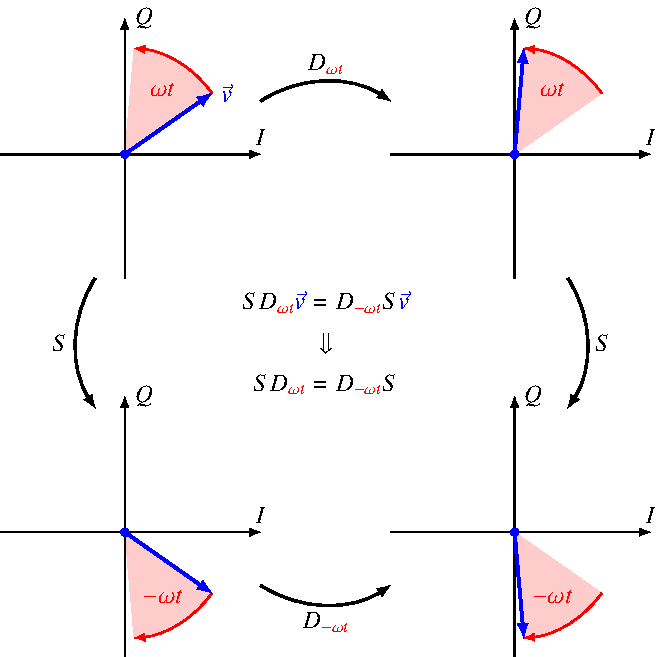
\includegraphics{applications/qam/images/spiegelung.pdf}
\caption{Vertauschungsregel für die Drehmatrizen $D_{\pm\omega t}$ und
die Matrix $S$ der Spiegelung an der $I$-Achse.
\label{figure:qam:spiegelung}}
\end{figure}
Zusammen bewirken sie dasselbe wie eine Drehung um $\omega t$ gefolgt
von einer Spiegelung an der $I$-Achse, also
\[
D_{-\omega t}S=SD_{\omega t}.
\]
Damit erhalten wir
\[
D_{-\omega t}PD_{\omega t}
=
\frac12E + \frac12 SD_{2\omega t},
\]
woraus wieder die Formel~\eqref{eqn:qam:filter}
für $\hat{v}(t)$ folgt.

\subsubsection{Filterung des Trägers}
\begin{figure}
\centering
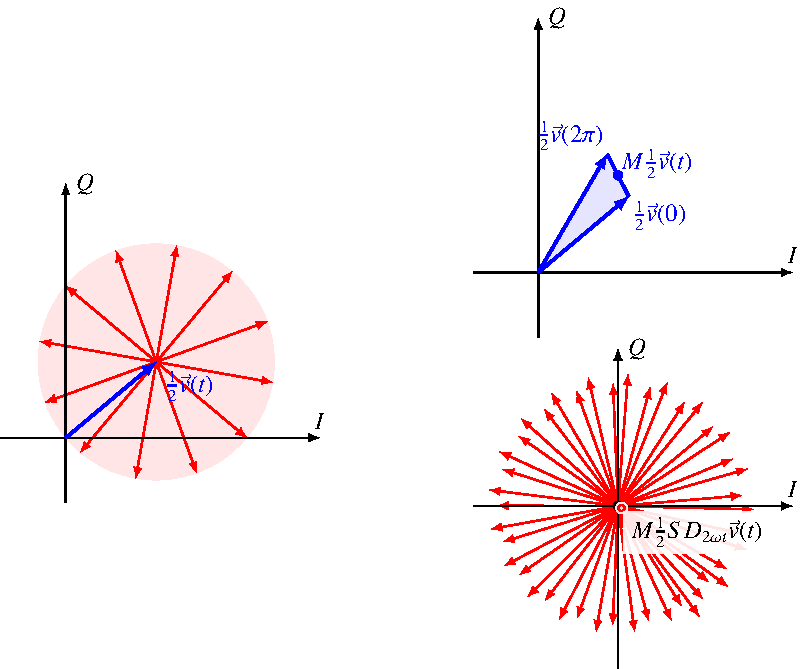
\includegraphics{applications/qam/images/filter.pdf}
\caption{Filterung des Trägers aus~\eqref{eqn:qam:filter}
links für ein konstantes Signal $\vec{v}(t)=\vec{v}(0)$, rechts
für ein langsam veränderliches Signal.
Zur besseren Lesbarkeit sind rechts die Terme
$\frac12\vec{v}(t)$ oben und $\frac12SD_{2\omega t}\vec{v}(t)$
unten getrennt.
Der Mittelwerte $\mathcal{M}\frac12SD_{2\omega t}$ ist der Beitrag des
zweiten Terms zum Mittelwert und sehr nahe beim Nullpunkt,
die Mittelung über ein Periodenintervall des Trägers bringt die
Trägerkomponente also fast vollständig zum Verschwinden.
\label{figure:qam:filter}}
\end{figure}
Gehen wir davon aus, dass die Bewegung des Vektors $\vec{v}(t)$ in
der $I$-$Q$-Ebene sehr viel langsamer ist als die Drehung mit der
Winkelgeschwindigkeit $2\omega$, dann können wir den zweiten Term
näherungsweise eliminieren.
Um dies zu verstehen, nehmen wir an, dass $\vec{v}(t)$ während eines
Zeitintervalls der Länge $L=\pi/\omega$ konstant ist ist.
Wir bezeichnen Mittelwerte über das Intervall mit dem Buchstaben $\mathcal{M}$.
Wir beachten dann, dass der zweite Term in \eqref{eqn:qam:filter}
für dieses Zeitintervall die gleichförmige, ganze Drehung des Vektors
um den Nullpunkt beschreibt.
Der Mittelwert des zweiten Terms über das Intervall verschwindet daher:
\[
\mathcal{M}\frac12SD_{2\omega t}\vec{v}(t)
=
0
\]
(siehe auch Abbildung~\ref{figure:qam:filter} links).
Der erste Term von \eqref{eqn:qam:filter} ist während des Intervalls
konstant, ihr Mittelwert ist daher
\[
\mathcal{M}\frac12\vec{v}(t)
=
\frac12\vec{v}(t).
\]
Wir finden daher den Mittelwert
\[
\mathcal{M}\hat{v}(t)
=
\frac12\vec{v}(t),
\]
bis auf den Faktor $\frac12$ wird also $\vec{v}(t)$ durch die Mittelwertbildung
rekonstruiert.
Verändert sich $\vec{v}(t)$ während des Intervalls um einen Betrag
kleiner als $\varepsilon$ (Abbildung~\ref{figure:qam:filter} rechts),
dann kommt ein Fehler hinzu, der ebenfalls
von der Grössenordnung $\varepsilon$ ist.

In praktischen Anwendungen ist die Frequenz des Trägers mehrere
Grössenordnungen grösser als die typischen Frequenzen in $I(t)$ 
und $Q(t)$, die Annahme, dass sich $\vec{v}(t)$ während einer halben
Trägerperiode nicht ändert, ist daher mit grosser Genauigkeit erfüllt.
Die Mittelwertbildung wird technisch mit Hilfe eines Tiefpassfilters
realisiert.

\subsubsection{Demodulationsfehler}
Bis jetzt sind wir davon ausgegangen, dass wir die Frequenz und die
Phase des Trägersignals genau kennen.
Doch dies ist nicht korrekt.
Die Demodulation erfolgt im Empfänger, wo die Matrix $D_{\omega t}$
neu erzeugt werden muss.
Dabei kann es zu Fehlern in der Frequenz kommen.
Die Demodulation erfolgt also mit einer Matrix $D_{\omega_rt}$
mit einer möglicherweise von der Sendefrequenz $\omega$
abweichenden Frequenz $\omega_r=\omega+\Delta\omega$.
Das decodierte Signal ist dann
\begin{equation}
\begin{aligned}
\hat{v}(t)
&=
D_{-\omega_rt}PD_{\omega t}\vec{v}(t)
=
D_{-(\omega+\Delta\omega)t} ({\textstyle\frac12}E+{\textstyle\frac12}S)
D_{\omega t}\vec{v}(t)
=
\frac12D_{-\Delta\omega t}\vec{v}(t)
+
\frac12D_{-(\omega+\Delta\omega)t}SD_{\omega t}\vec{v}(t)
\\
&=
\frac12 D_{-\Delta\omega t}\vec{v}(t)
+
\frac12 SD_{(\omega +\Delta\omega) t}D_{\omega t}\vec{v}(t)
=
\frac12 D_{-\Delta\omega t}\vec{v}(t)
+
\frac12 SD_{(2\omega +\Delta\omega) t}\vec{v}(t)
\end{aligned}
\label{eqn:qam:demoomegar}
\end{equation}
Bei der Filterung des Trägers verschwindet der zweite Term.
Die Demodulation liefert also nicht den Vektor $\vec{v}(t)$, vielmehr
rotiert der demodulierte Vektor mit der Winkelgeschwindigkeit $\Delta\omega$.

Korrekte Demodulation ist also nur möglich, wenn Sender und Empfänger exakt
die gleiche Frequenz verwenden.
Der Empfänger kann versuchen, die korrekte Frequenz aus dem empfangenen
Signal zu extrahieren, oder Sender und Empfänger können ein hochgenaues
Frequenznormal verwenden.
Ein Rubidium-Frequenznormal stellt eine Referenz-Frequenz mit einem
typischen relativen Fehler kleiner als $10^{-9}$ zur Verfügung.
Bei einem Trägersignal im typischen Bereich der Mobiltelefonie (Grössenordnung
$\sim 1\,\text{GHz}$) resultiert also weniger als eine Umdrehung von $\hat{v}(t)$
pro Sekunde.

Selbst wenn Sender und Empfänger hochgenaue Frequenzreferenzen verwenden,
wenn man also annehmen darf, dass $\omega_r=\omega$,
ist noch nicht sichergestellt, dass auch die Phase übereinstimmt.
Die Demodulation könnte mit einer um den Winkel $\delta$
phasenverschobenen Drehmatrix $D_{\omega t+\delta}$ erfolgen.
Die selbe Rechnung wie in \eqref{eqn:qam:demoomegar} liefert dann
\[
\hat{v}(t)
=
\frac12D_{-\delta}\vec{v}(t)
+
\frac12SD_{\delta+2\omega t}\vec{v}(t).
\]
Bei der Filterung fällt auch hier der zweite Term weg, der demodulierte
Vektor ist aber um den Winkel $-\delta$ verdreht.
Um dies zu vermeiden muss der Sender dem Empfänger die genaue Phase
irgendwie mitteilen.
Technische Möglichkeiten dazu werden in den nachstehenden Beispielen
kurz angesprochen.








%
% beispiele.tex
%
% (c) 2020 Prof Dr Andreas Müller, Hochschule Rapperswil
%
\subsection{Beispiele
\label{subsection:qam:beispiele}}
Die Quadratur-Amplituden-Modulation ermöglicht, im Vergleich zur
Trägerfrequenz langsam veränderliche zweidimensionale Signale zu
übertragen und wieder zu rekonstruieren.
Der besondere Nutzen dieser Technik ist jedoch, dass sie viele
ältere Modulationsverfahren als Spezialfälle enthält, wie in
diesem Abschnitt gezeigt werden soll.

\subsubsection{Amplitudenmodulation}
{\em Amplitudenmodulation} konnten wir verstehen, bevor wir $Q(t)$ kannten,
sie ist der Spezialfall $Q(t)=0$.
Für ein Audiosignal $A(t)$ mit $A(t)<1$ wird $I(t)=1+A(t)$ verwendet.
Das in Europa weitgehend bereits durch Digitalradio ersetzte 
Mittelwellenradio (AM) verwendet Amplitudenmodulation.
Bis 2025 werden in Europa alle Radiostationen digitalisiert, damit
wird AM für den Rundfunk aussterben.

\subsubsection{Phasenmodulation}
\begin{figure}
\centering
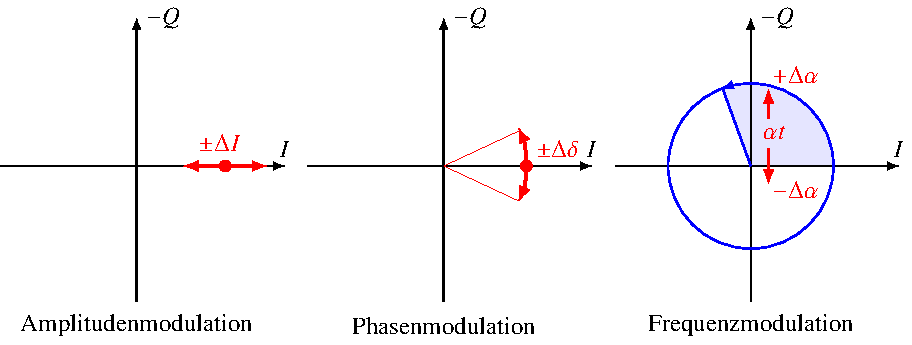
\includegraphics{applications/qam/images/amfmpm.pdf}
\caption{Amplitudenmodulation (links), Phasenmodulation (mitte) und
Frequenzmodulation in der $I$-$Q$-Ebene.
Frequenzmodulation ensteht durch eine Drehung in der $I$-$Q$-Ebene
mit der Kreisfrequenz der gewünschten Frequenzänderung.
\label{qam:figure:amfmpm}}
\end{figure}
Statt der Amplitude kann auch die Phase des Trägersignals moduliert werden.
Dazu muss $\omega t$ ersetzt werden durch $\omega t + \delta$.
Der konstante unmodulierte Vektor $\vec{v}_0$ in der $I$-$Q$-Ebene erzeugt
das modulierte Signal
\begin{align*}
D_{\omega t + \delta}
\vec{v}_0
&=
D_{\omega t}\underbrace{D_{\delta} \vec{v}_0}_{\displaystyle=\vec{v}(t)}.
\end{align*}
Eine Phasenänderung um den Winkel $\delta$ entsteht also dadurch, dass
man den Vektor $\vec{v}_0$ in der $I$-$Q$-Eben um $\delta$ dreht.
Dieses Modulationsverfahren heisst {\em Phasenmodulation}.
Abbildung~\ref{qam:figure:amfmpm} zeigt in der Mitte die Transformation
in der $I$-$Q$-Ebene, die Phasenmodulation bewirkt.

Mit reiner Amplitudenmodulation lässt sich kein Stereosignal übertragen.
Sind $L(t)$ und $R(t)$ die beiden Stereokanäle, dann erfolgt die
Amplitudenmodulation typischerweise mit $I(t)=1+L(t)+R(t)$,
wobei man wieder $L(t)+R(t)<1$ voraussetzen muss.
Ein reiner AM-Empfänger wird also nur das Audio-Signal $A(t)=L(t) + R(t)$
empfangen.

Um die Stereoinformation zu übermitteln, muss zusätzlich die Differenz
$L(t)-R(t)$ übermittelt werden.
Das C-QUAM Verfahren ({\bf C}ompatible {\bf Qu}adrature {\bf A}mplitude
{\bf M}odulation) verwendet dafür $Q(t)=L(t)-R(t)$.
Man darf annehmen, dass $L(t)-R(t)$ klein ist.
Dann befinden sich die Punkte $(I(t),Q(t))$ immer in der
Nähe der $I$-Achse, was sich in einer kleinen Verschiebung
\[
\delta = \arctan\frac{Q(t)}{I(t)} = \arctan\frac{L(t)-R(t)}{1+L(t)+R(t)}
\]
der Phase des übermittelten Signals äussert.
Der Betrag des Vektors $\vec{v}(t)$ ist dagegen
\begin{align*}
|\vec{v}(t)|
&=
\sqrt{
(1+L(t)+R(t))^2
+
(L(t)-R(t))^2
}
=
(1+L(t)+R(t))
\sqrt{
1+
\biggl(
\frac{L(t)-R(t)}{1+L(t)+R(t)}\biggr)^2
}
\\
&\simeq 1+L(t)+R(t),
\end{align*}
weil der zweite Summand unter der Wurzel klein ist.
Die $Q$-Komponente ändert also nicht wirklich etwas am Signal, welches
ein AM-Empfänger empfängt.

Um dem Emfpänger zu signalisieren, dass eine Stereoübertragung
vorliegt, wird $Q(t)$ zusätzlich ein Pilotton von 25\,Hz hinzugefügt.
Da nicht C-QUAM-taugliche Empfänger die Phasenschwankungen nicht erkennen
können, werden sie vom Pilotton auch nicht gestört.

\subsubsection{Frequenzmodulation}
Bei der {\em Frequenzmodulation} des UKW-Radios wird die Trägerfrequenz
im Takt des zu übertragenden Tonsignals verändert.
Lässt sich dies auch mit Hilfe der Signale $I(t)$ und $Q(t)$
beschreiben?
Welche Funktionen $I(t)$ und $Q(t)$ muss man wählen?

Ist das zu übertragende Audiosignal $0$, dann wird nur der unveränderte
Träger ausgestrahlt.
Dies lässt sich dadurch erreichen, dass man für $\vec{v}(t)$ den
konstanten Vektor $\vec{v}(t)=\vec{v}_0=(1,0)^t$ wählt.

Das ausgestrahlte Signal $s(t)$ entsteht als erste Komponente
des Vektors $D_{\omega t}\vec{v}(t)$.
Für konstantes $\vec{v}(t)=\vec{v}_0$ oszilliert es mit der Kreisfrequenz
$\omega$.
Will man, dass es schneller oszilliert, dann muss die Frequenz $\omega$
erhöht werden.
Möchte man die Frequenz um $\alpha$ steigern, dann muss man $\omega$
durch $\omega+\alpha$ ersetzen.
Das modulierte Signal ist dann
\[
\begin{pmatrix}
s(t)\\c(t)
\end{pmatrix}
=
D_{(\omega+\alpha)t} \vec{v}_0
=
D_{\omega t} \underbrace{D_{\alpha t} \vec{v}_0}_{\displaystyle=\vec{v}(t)}.
\]
Dies ist gleichbedeutend damit, dass man den Vektor $\vec{v}_0$ in der
$I$-$Q$-Ebene mit der Winkelgeschwindigkeit $\alpha$ dreht und so
$\vec{v}(t)$ erhält.
Daraus liest man ab, dass für die Signale $I(t)$ und $Q(t)$
\begin{equation}
\begin{pmatrix}I(t)\\Q(t)\end{pmatrix}
=
D_{\alpha t}\vec{v}_0
\qquad\Rightarrow\qquad
\left\{
\quad
\begin{aligned}
I(t)&=\cos\alpha t\\
Q(t)&=\sin\alpha t
\end{aligned}
\right.
\end{equation}
gilt.
Insbesondere kann man auch die Frequenzmodulation mit der
Quadratur-Amplituden-Modulation realisieren.
Abbildung~\ref{qam:figure:amfmpm} zeigt rechts symbolisch die
Kreisbewegung in der $I$-$Q$-Ebene, die Frequenzmodulation bewirkt.

\subsubsection{Analoges Farbfernsehen}
Die Entwicklung des analogen Farbfernsehens sah sich vor die Aufgabe 
gestellt, zusätzlich zur bereits im Schwarz-Weiss-Fernsehen übertragenen
Helligkeit (Luminanz, Y) die Farbinformation zu übermitteln.
Üblich ist dabei die Verwendung des YUV-Farbraumes, für den die zusätzlichen
Signale $U=R-Y$ und $V=B-Y$ benötigt werden, welche die Farbinformation
codieren.
Für ein farbloses Bild sind $U=0$ und $V=0$.

Das Problem ist also, zusätzlich zum Luminanzbild, welches bereits
amplitudenmoduliert übertragen wird, den Farbvektor $(U,V)^t$ zu
übertragen.
Es liegt daher nahe, dafür die Quadratur-Amplituden-Modulation zu
verwenden.
Im in Europa üblichen PAL-System wurde für den Träger für das Farbsignal
die Frequenz 4.43361875\,MHz verwendet.
Da ein Phasenfehler im Empfänger zu einer Drehung des Farbvektors
und damit zu einer auffälligen Verschiebung der Farben auf dem Farbkreis
führen würde, muss der Sender dem Empfänger die genaue Phase mitteilen.
Am Anfang jeder Zeile wird daher eine etwa zehn Perioden langer ``PAL-Burst''
übermittelt, den der Empfänger dazu verwenden kann, die Phase des
Farbträgers zu bestimmen.

Zusätzlich invertiert das PAL-System die Phase des Farbträgers
aufeinanderfolgender Zeilen, so dass sich Farbfehler durch Phasenfehler
auf aufeinanderfolgenden Zeilen wegmitteln.
Im PAL-System steht also Farbinformation jeweils nur für Paare von Zeilen
zur Verfügung und nur mit einer Dichte, die durch die Frequenz des Farbträgers
begrenzt ist.
Die effektive Farbauflösung eines PAL-Farbfernsehbildes ist daher halb so
gross wie die Helligkeitsauflösung.
Da auch die Farbauflösung des menschlichen Auges kleiner ist als die
Helligkeitsauflösung, ist diese Einschränkung des Systems von Auge nicht 
erkennbar.

\subsubsection{FSK und PSK}
Für die digitale Signalübertragung braucht man minimal die Fähigkeit,
zwei Zustände zu übermitteln, die man aber exakt wiedererkennnen können muss.
Frequency-Shift-Keying (FSK) ist ein Verfahren, welches zwei digitale Zustände
durch verschiedene Frequenzen codiert, es ist also ein
Frequenzmodulationsverfahren, von dem im vorangegangenen Abschnitt
bereits gezeigt wurde, wie es mit der Quadratur-Amplituden-Modulation
realisierbar ist.

Phase-Shift-Keying (PSK) verwendet stattdessen eine Phasenverschiebung
des Tragersignals.
Eine Phasenverschiebung um den Winkel $\varphi$ kann realisiert werden,
indem man eine Drehung um den Winkel $\varphi$ vorschaltet, also die
Drehmatrix $D_{\varphi}$ einfügt.
Besonders einfach ist eine Phasenverschiebung um den Winkel
$\varphi=180^\circ$, 
\[
D_{\varphi}
=
\begin{pmatrix}
\cos180^\circ&          - \sin180^\circ \\
\sin180^\circ& \phantom{-}\cos180^\circ
\end{pmatrix}
=
-E.
\]
Diese Phasenverschiebung wird also dadurch realisiert, dass man das
Vorzeichen von $I$ und $Q$ ändert.
Verwendet man den Vektor $(1,0)^t$ zur Codierung einer logischen
$\texttt{0}$, dann codiert der Vektor $(-1,0)^t$ eine logische $\texttt{1}$.
Auch PSK ist also mit Quadratur-Amplituden-Modulation realisierbar.

\subsubsection{Quantisierte QAM}
Mit Quadratur-Amplituden-Modulation lässt sich ein beliebiger Vektor
in der $I$-$Q$-Ebene übertragen.
Bei PSK wurden nur die Punkte $(1,0)$  und $(-1,0)$ in der $I$-$Q$-Ebene
verwendet.
Nach der Demodulation erhält man Vektoren, die wegen Fehlern nicht
exakt mit den ursprünglichen Vektoren übereinstimmen.
Da man aber nur die beiden logischen Zustände unterscheiden können muss,
kann man alle Vektoren mit $I>0$ als logische \texttt{0} decodieren
und Vektoren mit $I<0$ als logische \texttt{1}.

Statt nur zwei Zustände \texttt{0} und \texttt{1} zu codieren, könnte man
ein grössere Zahl von Punkten in der $I$-$Q$-Ebene verwenden, wie in
Abbildung~\ref{figure:qam:konstellation} dargestellt.
Die Punkte werden auch {\em Symbole} genannt.
Ein empfangener Vektor wird wegen Übertragungsfehlern nicht exakt mit
dem ursprünglichen Vektor übereinstimmen.
Zur Decodierung suchen wir dasjenige Symbol, welches dem Vektor am
nächsten liegt.
Man teilt also die Ebene in Teilgebiete $T_{\vec{v}_k}\subset \mathbb R^2$
zu jedem Symbol $\vec{v}_k$ auf.
Fällt der empfangene Vektor $\hat{v}$ in das Teilgebiet des Symbols
$\vec{v}_k$, also $\hat{v}\in T_{\vec{v}_k}$, dann decodieren wir ihn
als das Symbol $\vec{v}_k$.

\begin{figure}
\centering
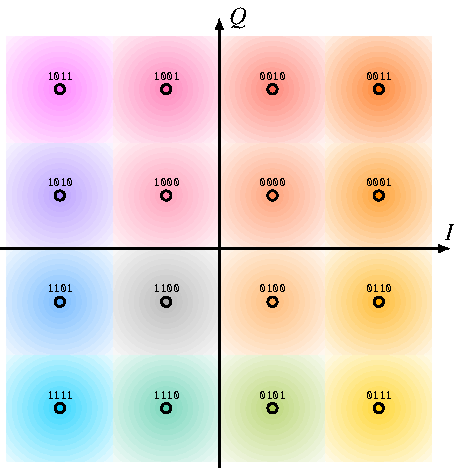
\includegraphics{applications/qam/images/konstellation.pdf}
\caption{Konstellationsdiagramm für quantisierte QAM mit 16 verschiedenen
Symbolen.
Mit jedem Symbol werden vier Bit codiert.
Zu jedem Symbol gehört ein quadratisches Gebiet gleicher Farbe.
Fällt der empfangene Vektor in eines dieser Gebiete, wird er als
das zugehörige Symbol decodiert.
\label{figure:qam:konstellation}}
\end{figure}

Im Beispiel der Abbildung~\ref{figure:qam:konstellation} können 16 
verschiedene Vektoren unterschieden werden, die man mit vierstelligen
Binärzahlen identifizieren kann.
Mit jedem Symbol werden also vier Bit übertragen.
Dieses Verfahren heisst auch 16-QAM und wird bei DVB-T verwendet.

Die Punkte-Menge $\vec{v}_k$ heisst auch die {\em Konstellation}
des Verfahrens.
Durch feinere Aufteilung können mehr Bits pro Symbol übertragen werden,
wie in Tabelle~\ref{table:qam:xqam} zusammengstellt.
Abbildung~\ref{figure:qam:analyzer} zeigt, wie sich die Messung eines 256-QAM 
Signals auf einem Vector Signal Analyzer darstellt.

Für ungerade Potenzen von $2$ kann das Konstellationsdiagramm kein
Quadrat sein.
Für $k$ ungerade kann man aber $2^k$ Punkte erhalten, indem man
dem Quadrat der $2^{k-1}$ Punkte der Konstellation von $2^{k-1}$-QAM
vier Rechtecke mit jeweils $2^{k-1}/4=2^{k-3}$ Punkten hinzugefügt, daraus
ergibt sich eine Konstellation mit
$2^{k-1}+4\cdot 2^{k-3}=2^{k-1}+2^{k-1}=2^k$
Punkten (Abbildung~\ref{qam:figure:qam-konstellation} Mitte).
In diesem hat das Konstellationsdiagramm also die Form
eines Kreuzes mit breite $2^{(k-1)/2}$ und Armlänge
$\frac32\cdot 2^{(k-1)/2}$.
Diese Konstellation wird manchmal auch Cross-QAM genannt.

\begin{table}
\centering
\begin{tabular}{rrcrl}
\hline
Bits&Symbole&Konstellation&Name&Anwendung\\
\hline
   2&      4&$  2\times   2$      &    4-QAM&DVB-S       \\
   4&     16&$  4\times   4$      &   16-QAM&V.29, DVB-T \\
   6&     64&$  8\times   8$      &   64-QAM&DVB-C, DVB-T\\
   8&    256&$ 16\times  16$      &  256-QAM&DVB-C       \\
  10&   1024&$ 32\times  32$      & 1024-QAM&            \\
  12&   4096&$ 64\times  64$      & 4096-QAM&DVB-C2, G.hn\\
  15&  32768&$128\times 256$ Kreuz&32767-QAM&ADSL        \\
\hline
\end{tabular}
\caption{Verschiedene Konstellationen für quantisierte QAM mit Anwendungen.
\label{table:qam:xqam}}
\end{table}

\begin{figure}
\centering
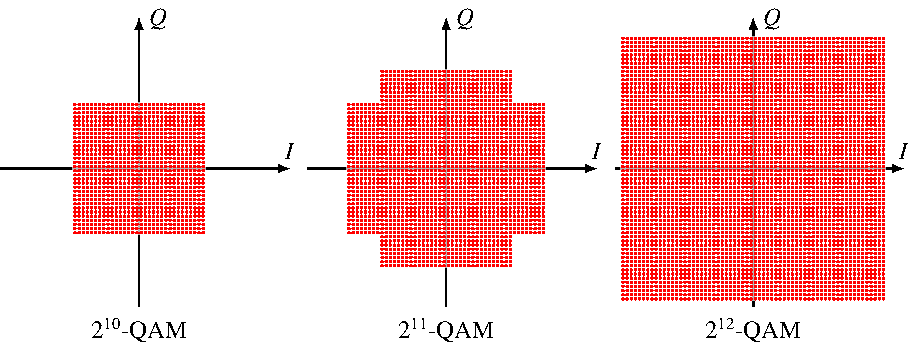
\includegraphics{applications/qam/images/qam.pdf}
\caption{Konstellationsdiagramme für $2^k$-QAM für verschiedene Werte von $k$.
\label{qam:figure:qam-konstellation}}
\end{figure}

\begin{figure}
\centering
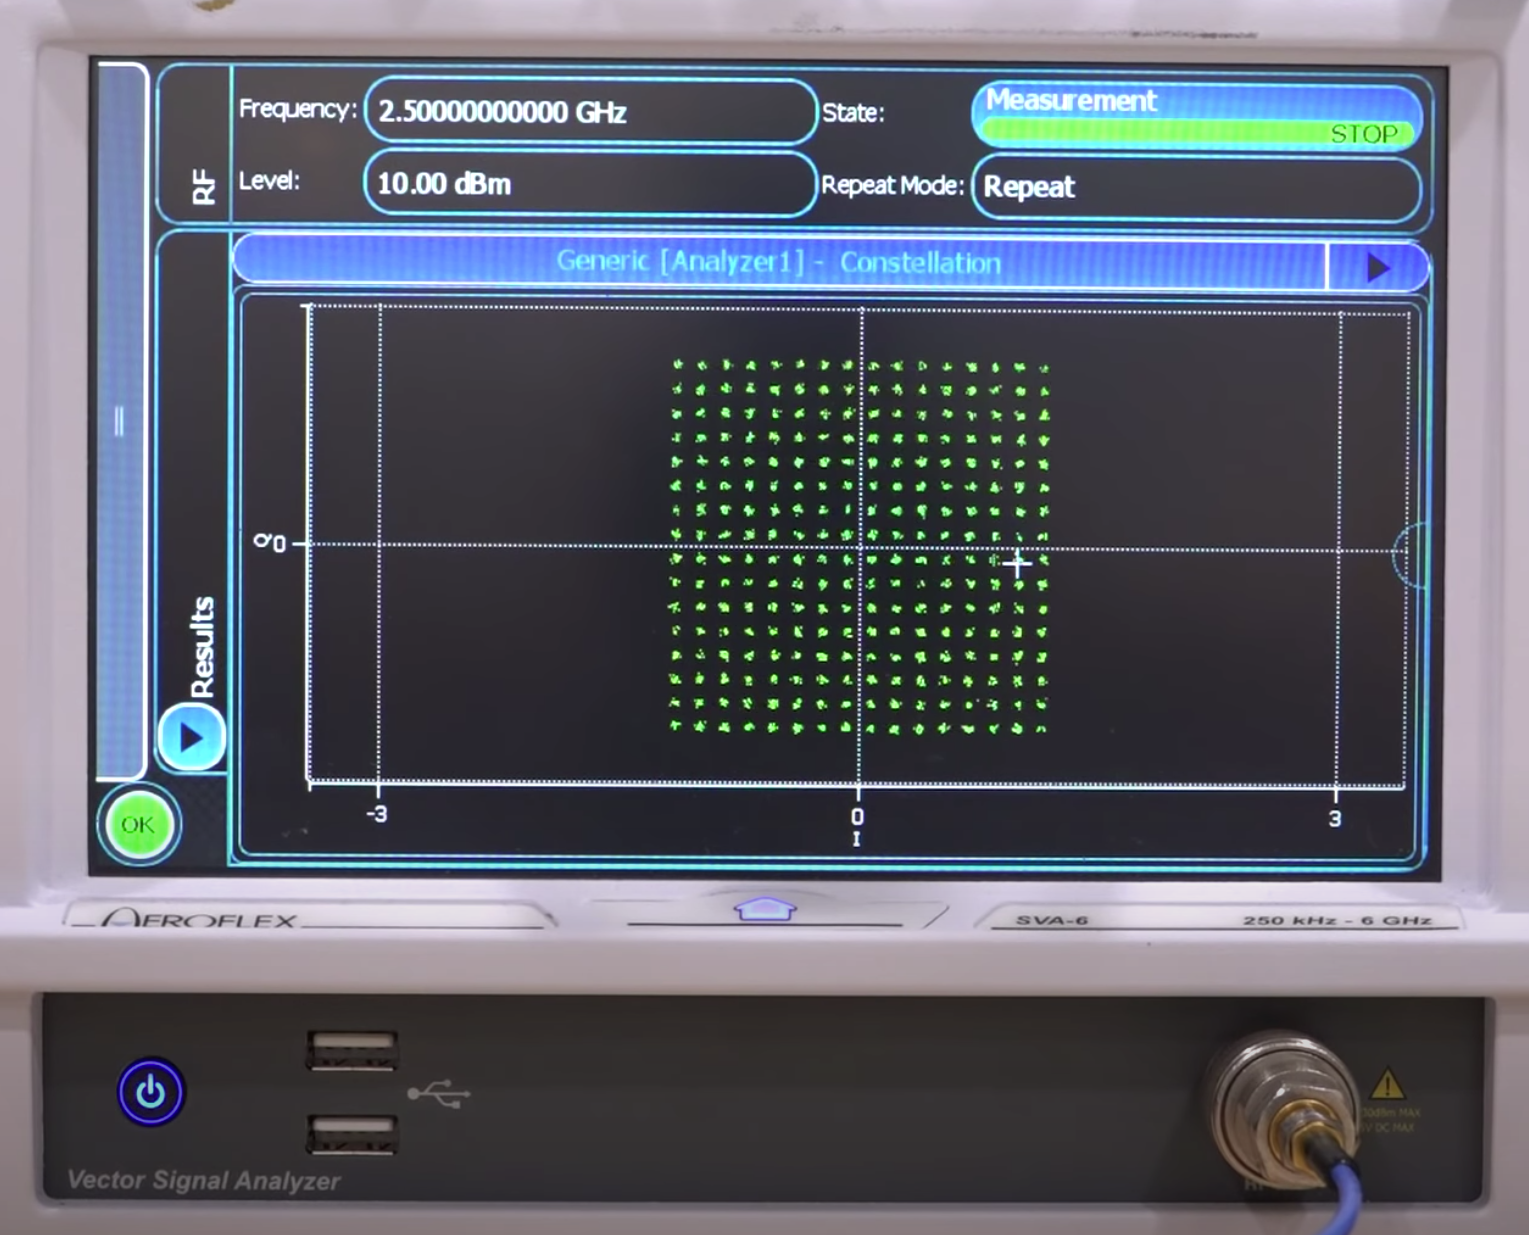
\includegraphics[width=1.0\hsize]{applications/qam/images/analyzer.png}
\caption{Messung des Konstellationsdiagramms eines 256-QAM Signals
mit einem Vector Signal Analyzer.
Man beachte die Beschriftung der Achsen mit \texttt{I} und \texttt{Q}.
(Ausschnitt aus dem Video \url{https://www.youtube.com/watch?v=uV3O3tpjmS8}
bei 26:36).
\label{figure:qam:analyzer}}
\end{figure}

\subsubsection{$n$-PSK}
Analog zum Vorgehen bei der quantisierten QAM kann auch PSK diskretisiert
werden.
Als Konstellationsdiagramm für $n$-PSK dienen $n$ Punkte auf einem Kreis,
die durch einen Winkel $2\pi/n$ getrennt sind.
In Abbildung~\ref{figure:qam:psk} ist das Konstellationsdiagramm für
$8$-PSK dargestellt.
\begin{figure}
\centering
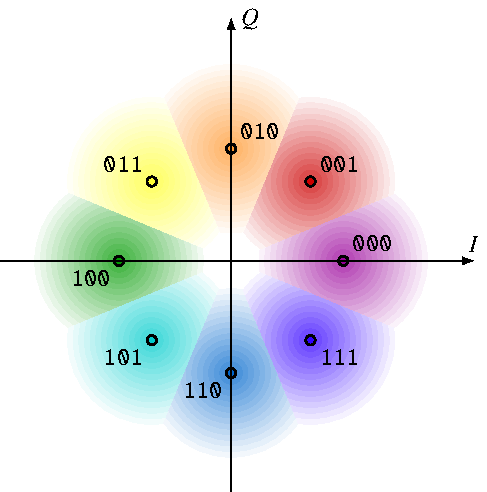
\includegraphics{applications/qam/images/psk.pdf}
\caption{Konstellationsdiagramm für 8-PSK 
\label{figure:qam:psk}}
\end{figure}

\subsubsection{Software Defined Radio}
Die vorangegangenen Beispiele haben illustriert, dass die
Quadratur-Amplituden-Modulation jedes besprochene Modulationsverfahren
realisieren kann.
Es ist nur nötig, einen Sender zu bauen, der Inputs $I(t)$ und $Q(t)$
entgegennimmt, die Modulation mit der Matrix $D_{\omega t}$ vornimmt
und das resultierende Signal $s(t)$ aussendet.
Auf der Empfängerseite braucht man eine physikalische Realisierung
der Matrix $D_{\omega_r t}$ und des Tiefpasses, der die demodulierten
Signal $\hat{I}(t)$ und $\hat{Q}(t)$ ausgibt.
Die Decodierung zum Beispiel als amplitudenmoduliertes Sprachsignal,
als frequenzmoduliertes Musiksignal oder als digitales 16-QAM-Signal
kann danach ausschliesslich in Software erfolgen.
Die Modulationsart eines solchen sogenannten {\em Software Defined Radio (SDR)}
wird also durch die Software definiert, welche die Signale $I(t)$ und $Q(t)$
erzeugt bzw.~die Signale $\hat{I}(t)$ und $\hat{Q}(t)$ analysiert.
SDR ermöglicht dem interessierten Hacker auch exotische Experimente,
wie das in Abbildung~\ref{qam:figure:digital} dargestellte fiktive
digitale Modulationsverfahren.

\begin{figure}
\centering

\includegraphics[width=0.7\hsize]{applications/qam/images/digital.jpg}
\caption{Konstellationsdiagramm für ein fiktives digitales
Modulationsverfahren, welches nur Punkte eines MathMan-Logos als
Symbole verwendet.
\label{qam:figure:digital}}
\end{figure}










